\clearpage

\section {2-flavour $\nu_{\mu}$-disappearance fits to the Run1, Run2 and Run1+2 datasets}
\label{sec:fits}

Using the method outlined in the previous sections and in Ref.\ \cite{OurRun1DisappAnalysis},
a 2-flavour $\nu_{\mu}$-disappearance fit was performed on the $1.431\times10^{20}$ POT Run1+2 dataset.
For GENIE, this analysis found
$|\Delta m^{2}_{23}|$ = 2.60$\times$10$^{-3}$ $eV^{2}/c^{4}$ and
$sin^{2}2\theta_{23}$ = 0.97 
to be the best-fit values ($\chi^{2}/ndf$=0.310).
For NEUT, the corresponding best-fit values were
$|\Delta m^{2}_{23}|$ = 2.65$\times$10$^{-3}$ $eV^{2}/c^{4}$ and
$sin^{2}2\theta_{23}$ = 0.98 ($\chi^{2}/ndf$=0.311).
The reconstructed neutrino energy distribution of the 31 single $\mu$-like ring events in the Run1+2 dataset, 
along with the best-fit predictions from GENIE and NEUT, are shown in  
Figs.\ \ref{fig:run1p2_spectrum_and_data_genie} and \ref{fig:run1p2_spectrum_and_data_neut}.
These distributions are shown in the 50 MeV reconstructed neutrino energy bins that were used in the fitting procedure.
It is illuminating to see the same distributions with a smaller number of bins of
 variable size in reconstructed neutrino energy; these are shown in 
Figs.\ \ref{fig:run1p2_spectrum_and_data_genie_rebin} and \ref{fig:run1p2_spectrum_and_data_neut_rebin}, 
though this binning scheme was not used in the analysis.
In Figs.\ \ref{fig:run1p2_spectrum_and_data_genie_rebin_modes} and \ref{fig:run1p2_spectrum_and_data_neut_rebin_modes},
the $\nu_{\mu}$-CCQE component of the best-fit oscillation hypothesis is added to the distributions shown in the previous figures.

The $\Delta\chi^{2}$ distributions
for the fit to the Run1+2 dataset are shown as a function of $sin^{2}2\theta_{23}$ and $|\Delta m^{2}_{23}|$ in
Fig.\ \ref{fig:run1p2_genie_deltachisqsurf_wide} for GENIE and
Fig.\ \ref{fig:run1p2_neut_deltachisqsurf_wide} for NEUT.
Meanwhile zoomed views around the Run1+2 best-fit values of these $\Delta\chi^{2}$ distributions are shown in
Fig.\ \ref{fig:run1p2_genie_deltachisqsurf_zoom} for GENIE and
Fig.\ \ref{fig:run1p2_neut_deltachisqsurf_zoom} for NEUT.
The marginalised $\Delta\chi^{2}$ distributions for the Run1+2 fit are shown in
Fig.\ \ref{fig:run1p2_genie_marginal_deltachisq_wide} for GENIE and
Fig.\ \ref{fig:run1p2_neut_marginal_deltachisq_wide} for NEUT.
The 1-dimensional marginalised $\Delta\chi^{2}$ distributions are obtained by minimizing $\Delta\chi^{2}$ with respect to
$sin^{2}2\theta_{23}$ for each $|\Delta m^{2}_{23}|$ bin (and vice versa).

Comparisons of the Run1+2 best-fit values with distributions obtained by
2-flavour $\nu_{\mu}$-disappearance 
fits on 1.431$\times$10$^{20}$ POT toy MC experiments 
generated with $sin^{2}2\theta_{23}$ = 1.0 and 
$|\Delta m^{2}_{23}|$ = 2.32$\times10^{-3}$ $eV^{2}/c^{4}$ are shown 
in Figs. \ref{fig:genie-minos11-run1p2-toymc-chisq-distribution} and 
\ref{fig:genie-minos11-run1p2-toymc-bestfitparam-distributions} for GENIE and
in Figs. \ref{fig:neut-minos11-run1p2-toymc-chisq-distribution} and 
\ref{fig:neut-minos11-run1p2-toymc-bestfitparam-distributions} for NEUT.

For comparison, we performed the same 2-flavour $\nu_{\mu}$-disappearance fit separately on the 
$0.323\times10^{20}$-POT Run1 and $1.108\times10^{20}$-POT Run2 datasets.
A summary of the best-fit values for all fits is given in Table \ref{table:bestfit_params_summary}.
The reconstructed neutrino energy spectrum for Run1 (Run2) 1 $\mu$-like ring events 
along with the best-fit and null hypothesis predictions from GENIE are shown in 
Fig.\ \ref{fig:run1_spectrum_and_data_genie_rebin_modes} (Fig.\ \ref{fig:run2_spectrum_and_data_genie_rebin_modes}).
The corresponding Run1 (Run2) distributions for NEUT are shown in
Fig.\ \ref{fig:run1_spectrum_and_data_neut_rebin_modes} (Fig.\ \ref{fig:run2_spectrum_and_data_neut_rebin_modes}).

The marginalised $\Delta\chi^{2}$ distributions for the 2-flavour
$\nu_{\mu}$-disappearance fits to the Run1, Run2 and the combined Run1+2 datasets are shown 
as a function of $sin^{2}2\theta_{23}$ in
Fig.\ \ref{fig:genie_deltachisq_sinsq2theta_3datasets} for GENIE and 
Fig.\ \ref{fig:neut_deltachisq_sinsq2theta_3datasets} for NEUT.
These distributions are also shown as a function of $|\Delta m^{2}_{23}|$ in 
Fig.\ \ref{fig:genie_deltachisq_dmsq_narrow_3datasets} for GENIE and
Fig.\ \ref{fig:neut_deltachisq_dmsq_narrow_3datasets} for NEUT 
(with $|\Delta m^{2}_{23}|$ restricted in the fit to the range
1$\times$10$^{-3}$ $eV^{2}/c^{4}$ - 6$\times$10$^{-3}$ $eV^{2}/c^{4}$).
The effects on these distributions of extending the $|\Delta m^{2}_{23}|$ range to
1$\times$10$^{-3}$ $eV^{2}/c^{4}$ - 30$\times$10$^{-3}$ $eV^{2}/c^{4}$ are
shown in
Fig.\ \ref{fig:genie_deltachisq_dmsq_wide_3datasets} for GENIE and
Fig.\ \ref{fig:neut_deltachisq_dmsq_wide_3datasets} for NEUT.

%
% Summary of best-fit params for the GENIE/NEUT fits to Run1,Run2,Run1+2 fits
%

\begin{table*}[htb]
\center
\renewcommand{\arraystretch}{1.75} % enlarge line spacing
\begin{tabular}{|c||c|c|}
\hline
Dataset                             &  GENIE best-fit values                                         &  NEUT best-fit values   \\
\hline
$0.323\times10^{20}$ POT Run1       &   $|\Delta m^{2}_{23}|$ = 2.77 $\times10^{-3}$ $eV^{2}/c^{4}$  &  $|\Delta m^{2}_{23}|$ = 2.88 $\times10^{-3}$ $eV^{2}/c^{4}$     \\
                                    &   $sin^{2}2\theta_{23}$ = 0.81                                 &  $sin^{2}2\theta_{23}$ = 0.84 \\
                                    &   $\chi^{2}/ndf$ = 0.105                                       &  $\chi^{2}/ndf$ = 0.114 \\
                                    &   (MINOS 2011 params $\chi^{2}/ndf$ = 0.121)                   &  (MINOS 2011 params $\chi^{2}/ndf$ = 0.129) \\
\hline
$1.108\times10^{20}$ POT Run2       &   $|\Delta m^{2}_{23}|$ = 2.59 $\times10^{-3}$ $eV^{2}/c^{4}$  &  $|\Delta m^{2}_{23}|$ = 2.62 $\times10^{-3}$ $eV^{2}/c^{4}$     \\
                                    &   $sin^{2}2\theta_{23}$ = 1.00                                 &  $sin^{2}2\theta_{23}$ = 1.00 \\
                                    &   $\chi^{2}/ndf$ = 0.318                                       &  $\chi^{2}/ndf$ = 0.310 \\
                                    &   (MINOS 2011 params $\chi^{2}/ndf$ = 0.327)                   &  (MINOS 2011 params $\chi^{2}/ndf$ = 0.322) \\
\hline
$1.431\times10^{20}$ POT Run1+2     &   $|\Delta m^{2}_{23}|$ = 2.60 $\times10^{-3}$ $eV^{2}/c^{4}$  &  $|\Delta m^{2}_{23}|$ = 2.65 $\times10^{-3}$ $eV^{2}/c^{4}$     \\
                                    &   $sin^{2}2\theta_{23}$ = 0.97                                 &  $sin^{2}2\theta_{23}$ = 0.98 \\
                                    &   $\chi^{2}/ndf$ = 0.310                                       &  $\chi^{2}/ndf$ = 0.311 \\
                                    &   (MINOS 2011 params $\chi^{2}/ndf$ = 0.319)                   &  (MINOS 2011 params $\chi^{2}/ndf$ = 0.322) \\
\hline
\end{tabular}\\[2pt]
\caption{
  Summary of best-fit parameter values for 2-flavour oscillation fits to the Run1, Run2 and the combined Run1+2 datasets.
  The $\chi^{2}/ndf$ ($ndf$=198) value is also given assuming the MINOS 2011 best-fit parameters
  ($sin^{2}2\theta_{23}$ = 1.0 and $|\Delta m^{2}_{23}|$ = 2.32$\times10^{-3}$ $eV^{2}/c^{4}$).
}
\label{table:bestfit_params_summary}
\end{table*}
  


%
% .....................................................................................................................
%

\clearpage

%
% Run1+2 fit data/best-fit distribution (50 MeV binning)
%

\begin{figure*}[htb]
\center
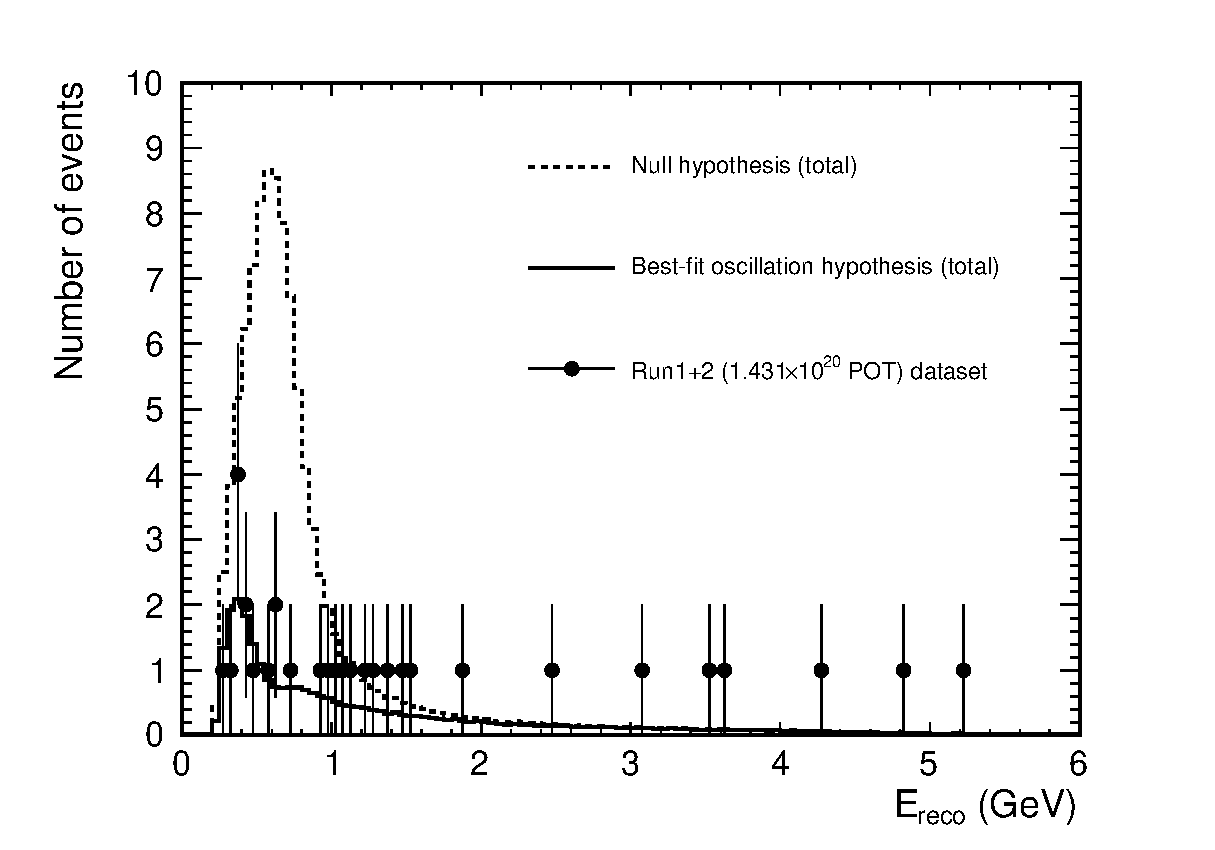
\includegraphics[width=30pc,height=19pc]{./images/fits/run1p2_genie_bestfit_spectrum.eps}
\caption{
  Reconstructed neutrino energy distribution of the 31 single $\mu$-like ring events of the combined
  1.431$\times$10$^{20}$ POT Run1+2 dataset (points) and GENIE best-fit SuperK prediction (solid line).
  The distributions are shown using the 50 MeV reconstructed neutrino energy binning used in the fitting procedure.
  The best-fit oscillation parameters are
  $|\Delta m^{2}_{23}|$ = 2.60$\times$10$^{-3}$ $eV^{2}/c^{4}$ and $sin^{2}2\theta_{23}$ = 0.97.
  The dotted line shows the GENIE prediction without oscillations.
}
\label{fig:run1p2_spectrum_and_data_genie}
\end{figure*}

\begin{figure*}[htb]
\center
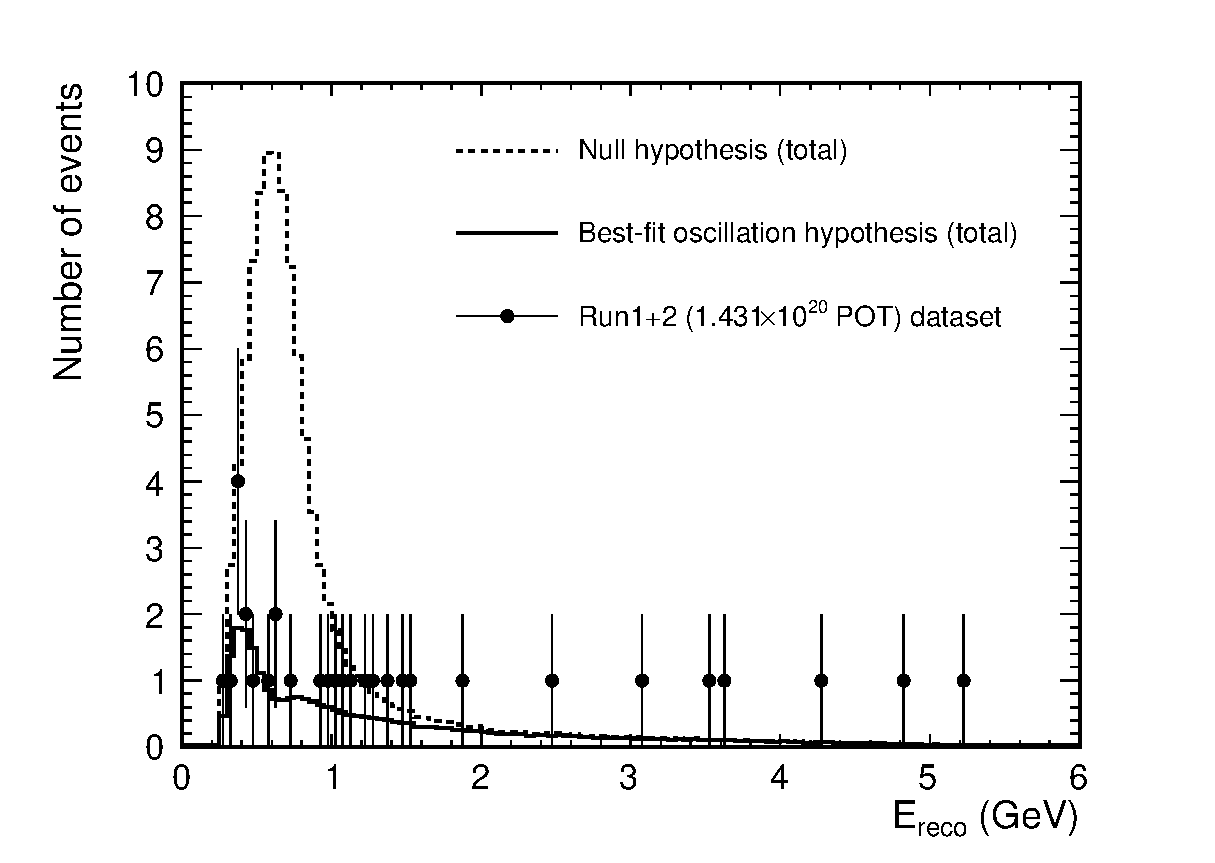
\includegraphics[width=30pc,height=19pc]{./images/fits/run1p2_neut_bestfit_spectrum.eps}
\caption{
  Reconstructed neutrino energy distribution of the 31 single $\mu$-like ring events of the combined
  1.431$\times$10$^{20}$ POT Run1+2 dataset (points) and NEUT best-fit SuperK prediction (solid line).
  The distributions are shown using the 50 MeV reconstructed neutrino energy binning used in the fitting procedure.
  The best-fit oscillation parameters are
  $|\Delta m^{2}_{23}|$ = 2.65$\times$10$^{-3}$ $eV^{2}/c^{4}$ and $sin^{2}2\theta_{23}$ = 0.98.
  The dotted line shows the NEUT prediction without oscillations.
}
\label{fig:run1p2_spectrum_and_data_neut}
\end{figure*}

%
% Run1+2 fit data/best-fit distribution (variable binning)
%

\begin{figure*}[htb]
\center
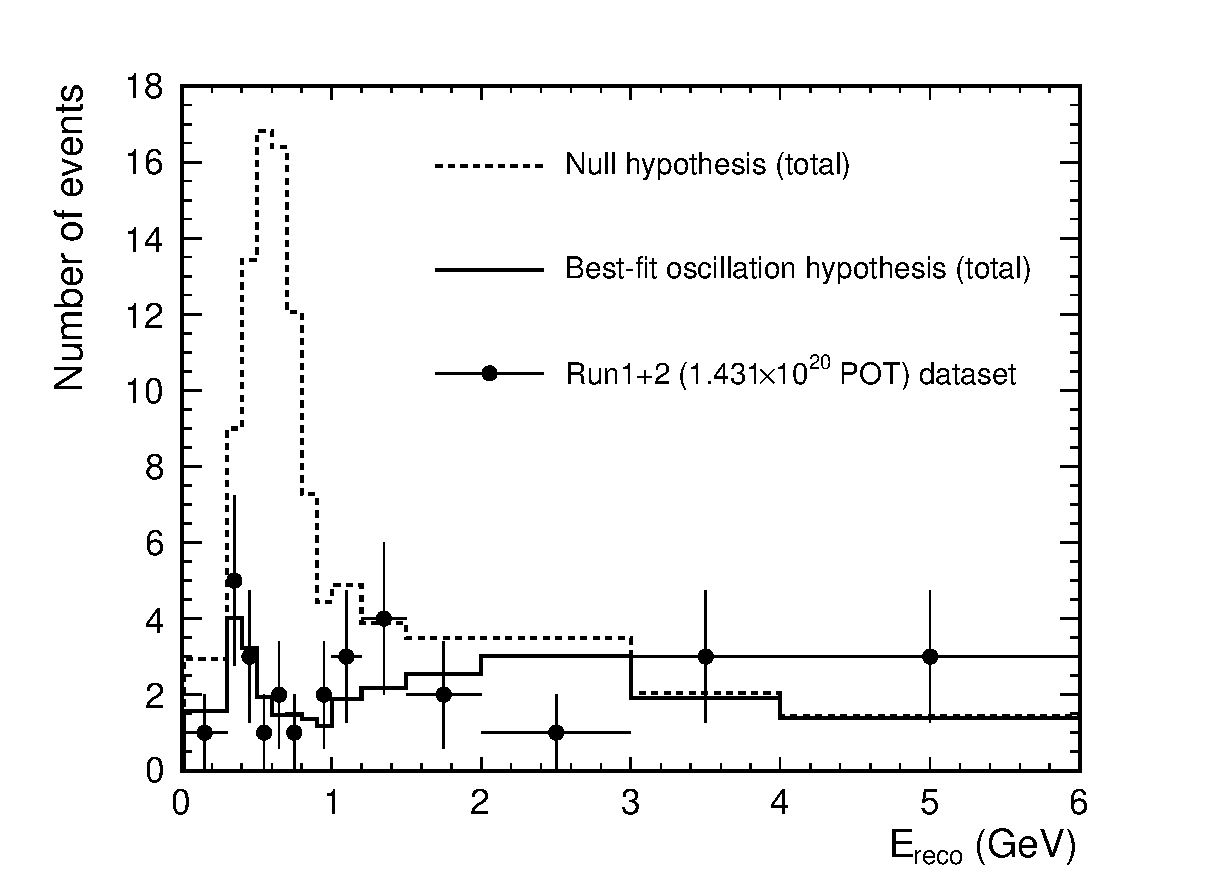
\includegraphics[width=32pc]{./images/fits/run1p2_genie_bestfit_spectrum_rebin.eps}
\caption{
  Reconstructed neutrino energy distribution of the 31 single $\mu$-like ring events of the combined
  1.431$\times$10$^{20}$ POT Run1+2 dataset (points) and GENIE best-fit SuperK prediction (solid line).
  The distributions are shown using a variable binning scheme; this is for illustration purposes only, 
  and this binning scheme was not used in the analysis.
  The best-fit oscillation parameters are
  $|\Delta m^{2}_{23}|$ = 2.60$\times$10$^{-3}$ $eV^{2}/c^{4}$ and $sin^{2}2\theta_{23}$ = 0.97.
  The dotted line shows the GENIE prediction without oscillations.
}
\label{fig:run1p2_spectrum_and_data_genie_rebin}
\end{figure*}

\begin{figure*}[htb]
\center
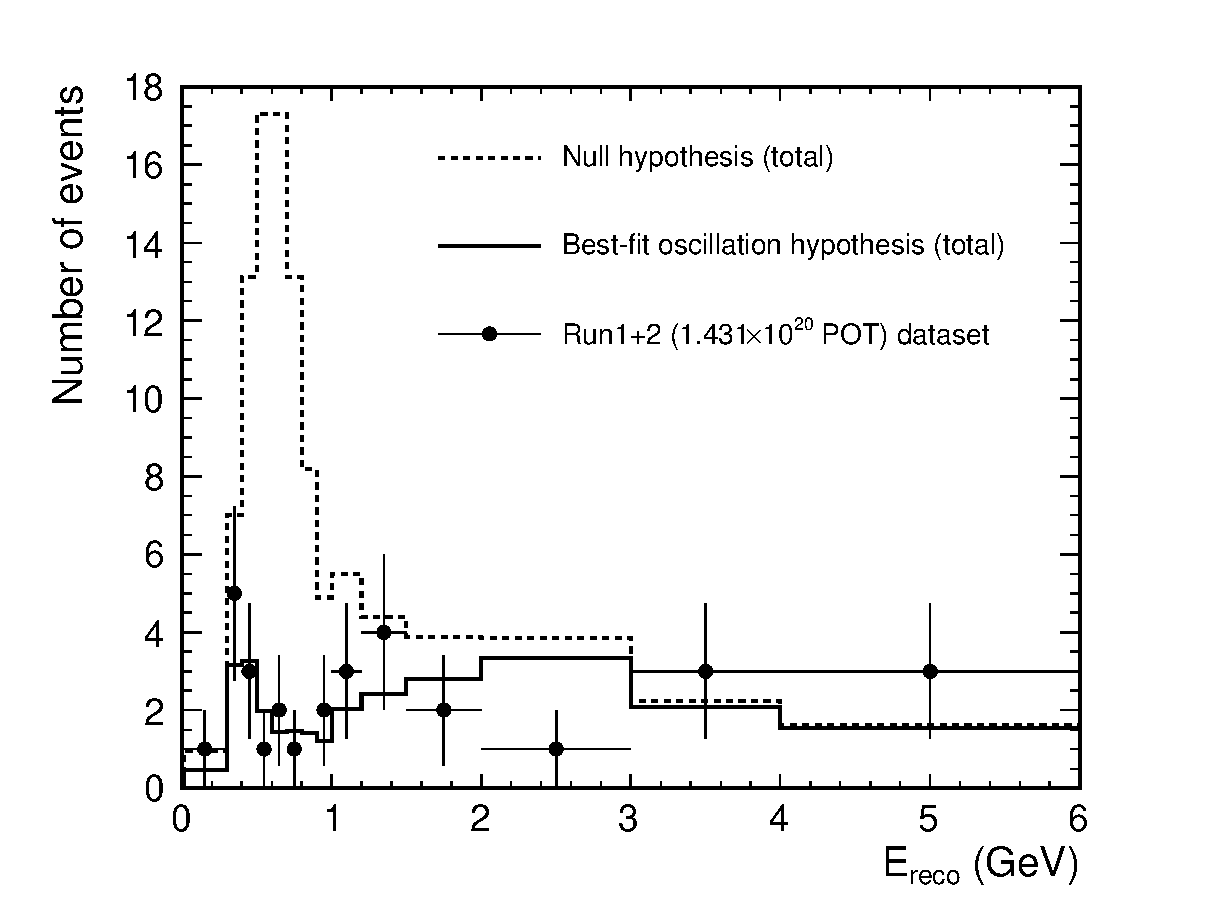
\includegraphics[width=32pc]{./images/fits/run1p2_neut_bestfit_spectrum_rebin.eps}
\caption{
  Reconstructed neutrino energy distribution of the 31 single $\mu$-like ring events of the combined
  1.431$\times$10$^{20}$ POT Run1+2 dataset (points) and NEUT best-fit SuperK prediction (solid line).
  The distributions are shown using a variable binning scheme; this is for illustration purposes only,
  and this binning scheme was not used in the analysis.
  The best-fit oscillation parameters are
  $|\Delta m^{2}_{23}|$ = 2.65$\times$10$^{-3}$ $eV^{2}/c^{4}$ and $sin^{2}2\theta_{23}$ = 0.98.
  The dotted line shows the NEUT prediction without oscillations.
}
\label{fig:run1p2_spectrum_and_data_neut_rebin}
\end{figure*}

%
% Run1+2 fit data/best-fit distribution (variable binning + CCQE/other)
%

\begin{figure*}[htb]
\center
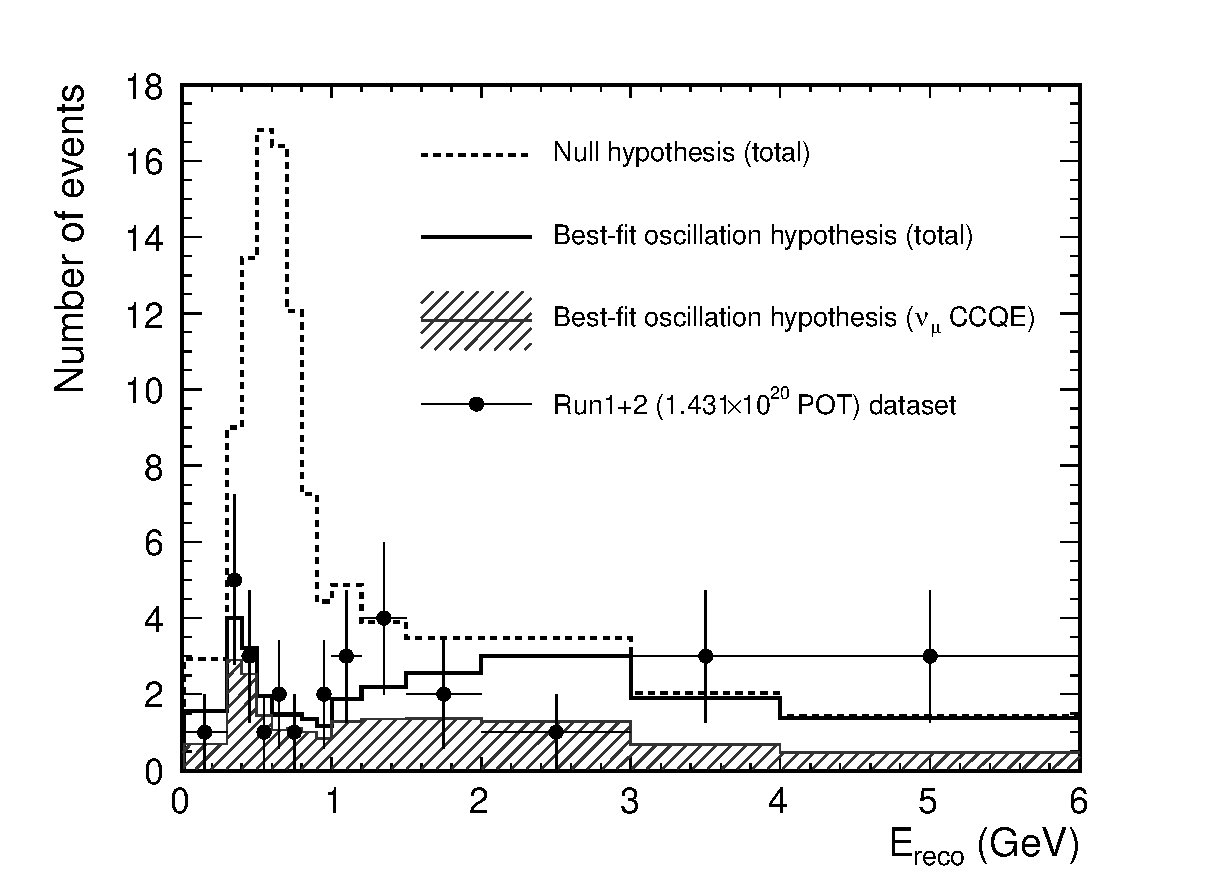
\includegraphics[width=32pc]{./images/fits/run1p2_genie_bestfit_spectrum_rebin_modes.eps}
\caption{
  Same distributions as in Fig.\ref{fig:run1p2_spectrum_and_data_genie_rebin} with the 
  addtion of the $\nu_{\mu}$-CCQE component of the best-fit oscillation hypothesis (GENIE)
}
\label{fig:run1p2_spectrum_and_data_genie_rebin_modes}
\end{figure*}

\begin{figure*}[htb]
\center
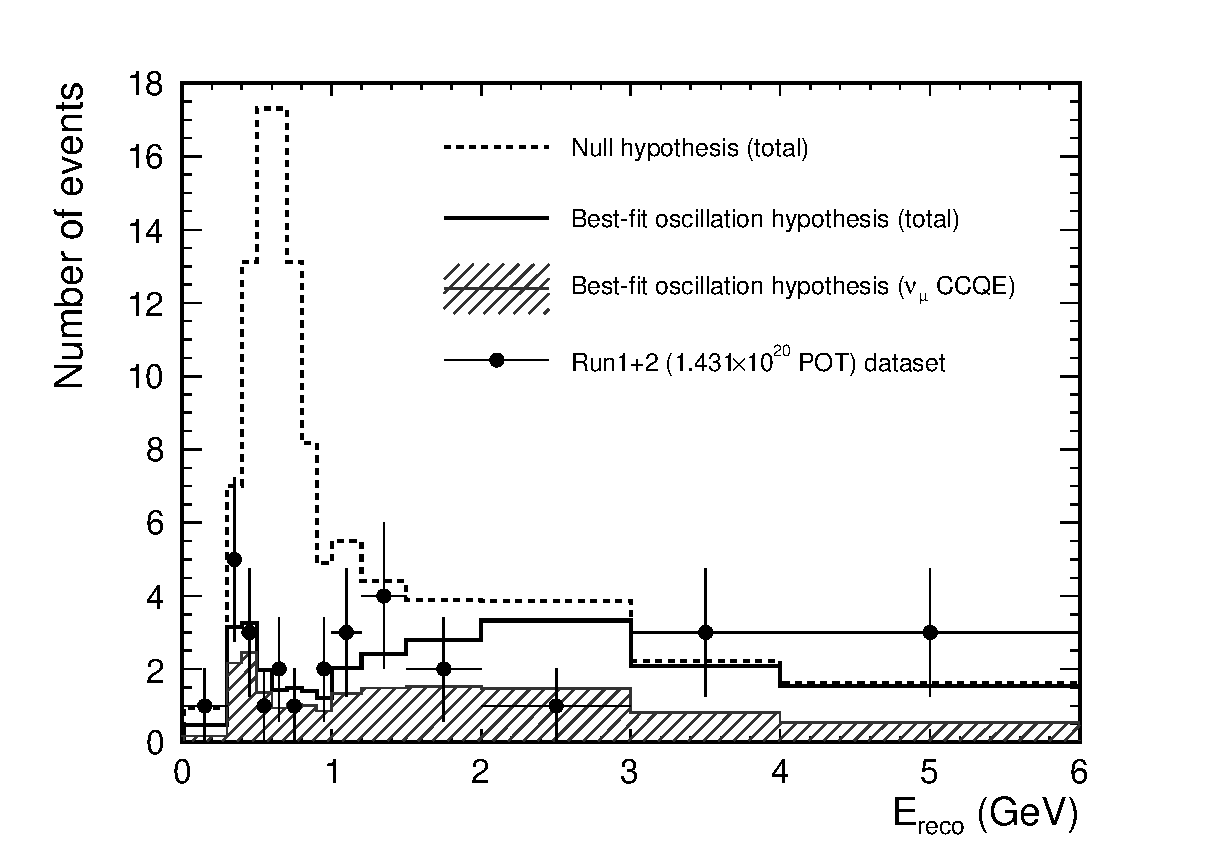
\includegraphics[width=32pc]{./images/fits/run1p2_neut_bestfit_spectrum_rebin_modes.eps}
\caption{
  Same distributions as in Fig.\ref{fig:run1p2_spectrum_and_data_neut_rebin} with the
  addition of the $\nu_{\mu}$-CCQE component of the best-fit oscillation hypothesis (NEUT)
}
\label{fig:run1p2_spectrum_and_data_neut_rebin_modes}
\end{figure*}


%
% Run1+2 delta chisq surfaces
%

\begin{figure}[ht]
\begin{minipage}[t]{0.47\linewidth}
\centering
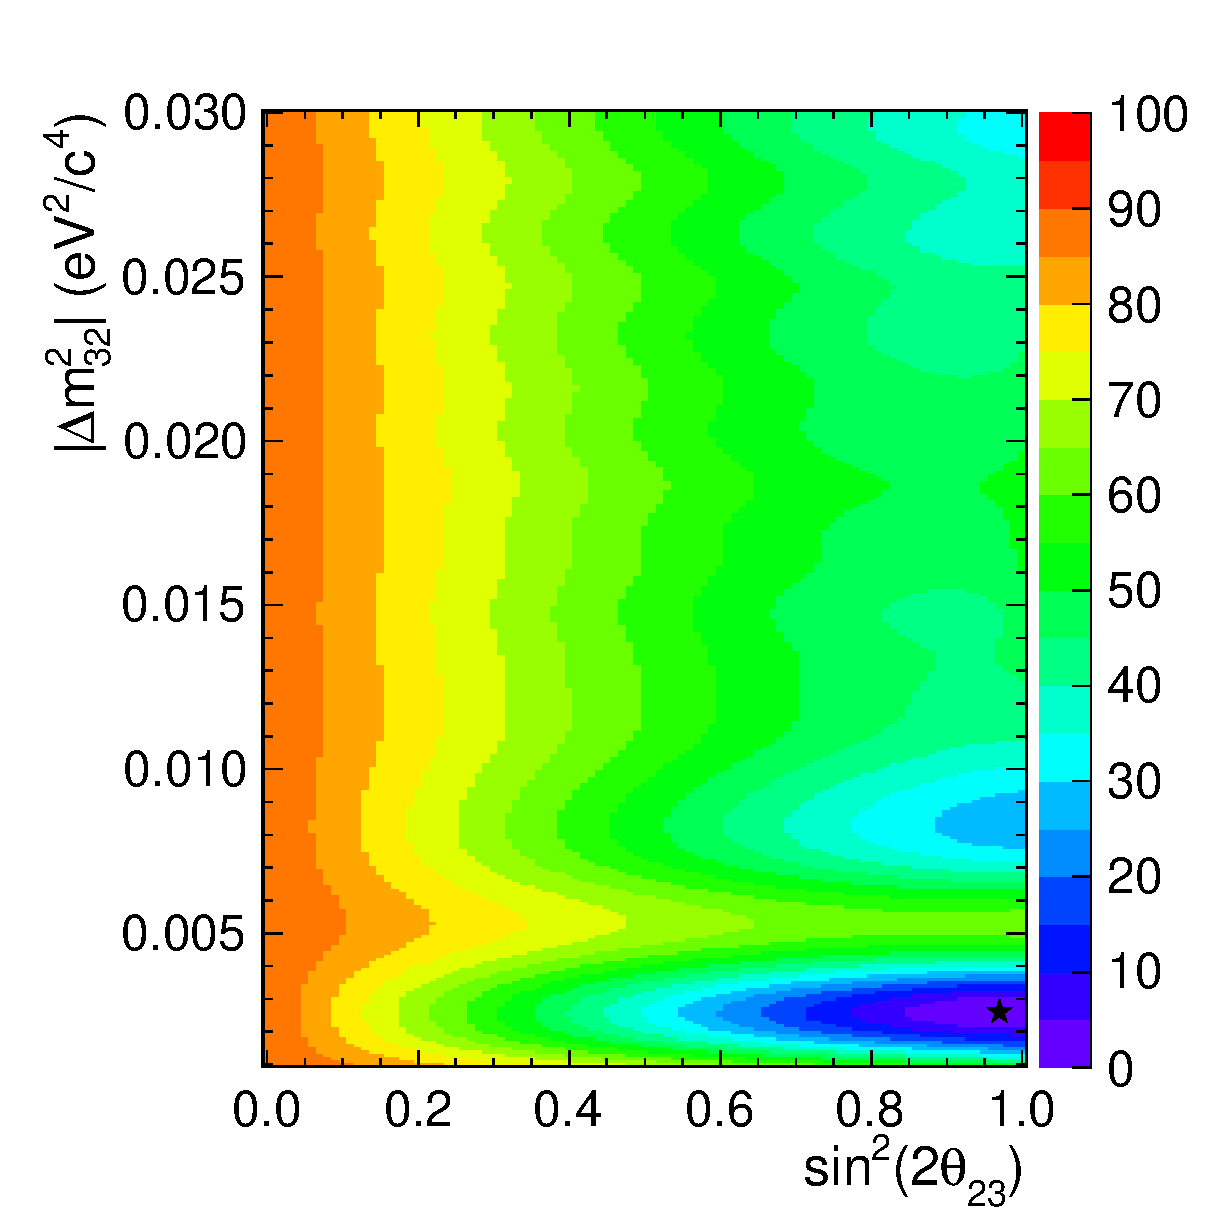
\includegraphics[width=18pc,height=19pc]{./images/fits/run1p2_genie_deltachisqsurf_wide.eps}
\caption{
  $\Delta\chi^{2}$ surface for the 2-flavour disappearance fit to the combined 1.431$\times$10$^{20}$ POT Run1+2 dataset (GENIE)
}
\label{fig:run1p2_genie_deltachisqsurf_wide}
\end{minipage}
\hspace{0.06\linewidth}
\begin{minipage}[t]{0.47\linewidth}
\centering  
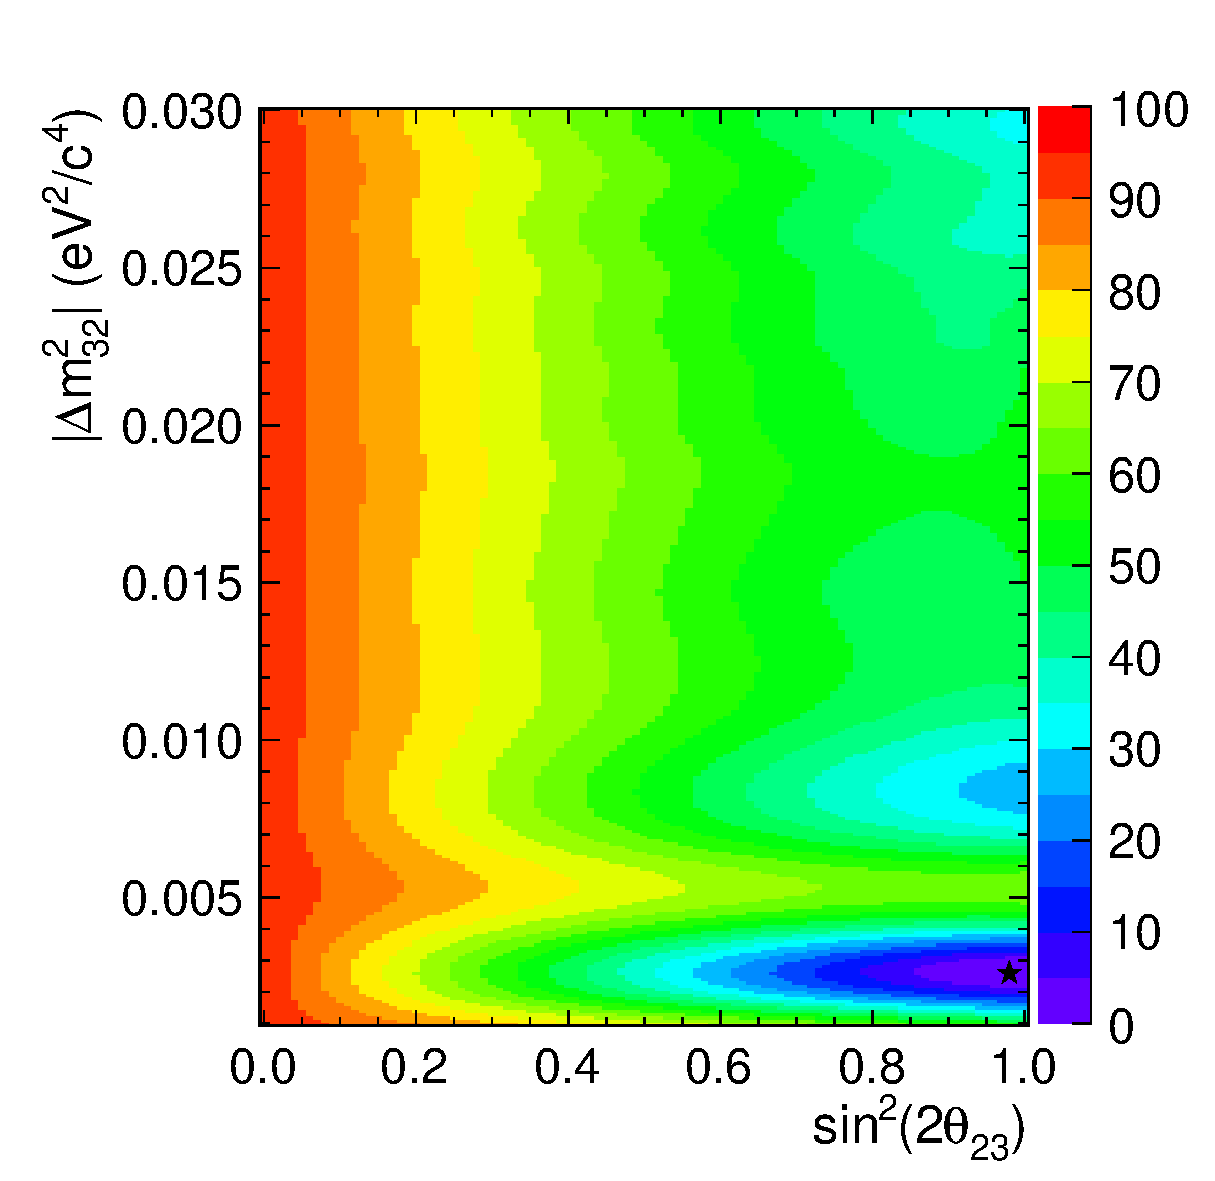
\includegraphics[width=18pc,height=19pc]{./images/fits/run1p2_neut_deltachisqsurf_wide.eps}
\caption{
  $\Delta\chi^{2}$ surface for the 2-flavour disappearance fit to the combined 1.431$\times$10$^{20}$ POT Run1+2 dataset (NEUT)
}
\label{fig:run1p2_neut_deltachisqsurf_wide}
\end{minipage}
\end{figure}

%
% Run1+2 delta chisq surfaces (zoomed around MINOS-2011 best-fit values)
%

\begin{figure}[ht]
\begin{minipage}[t]{0.47\linewidth}
\centering
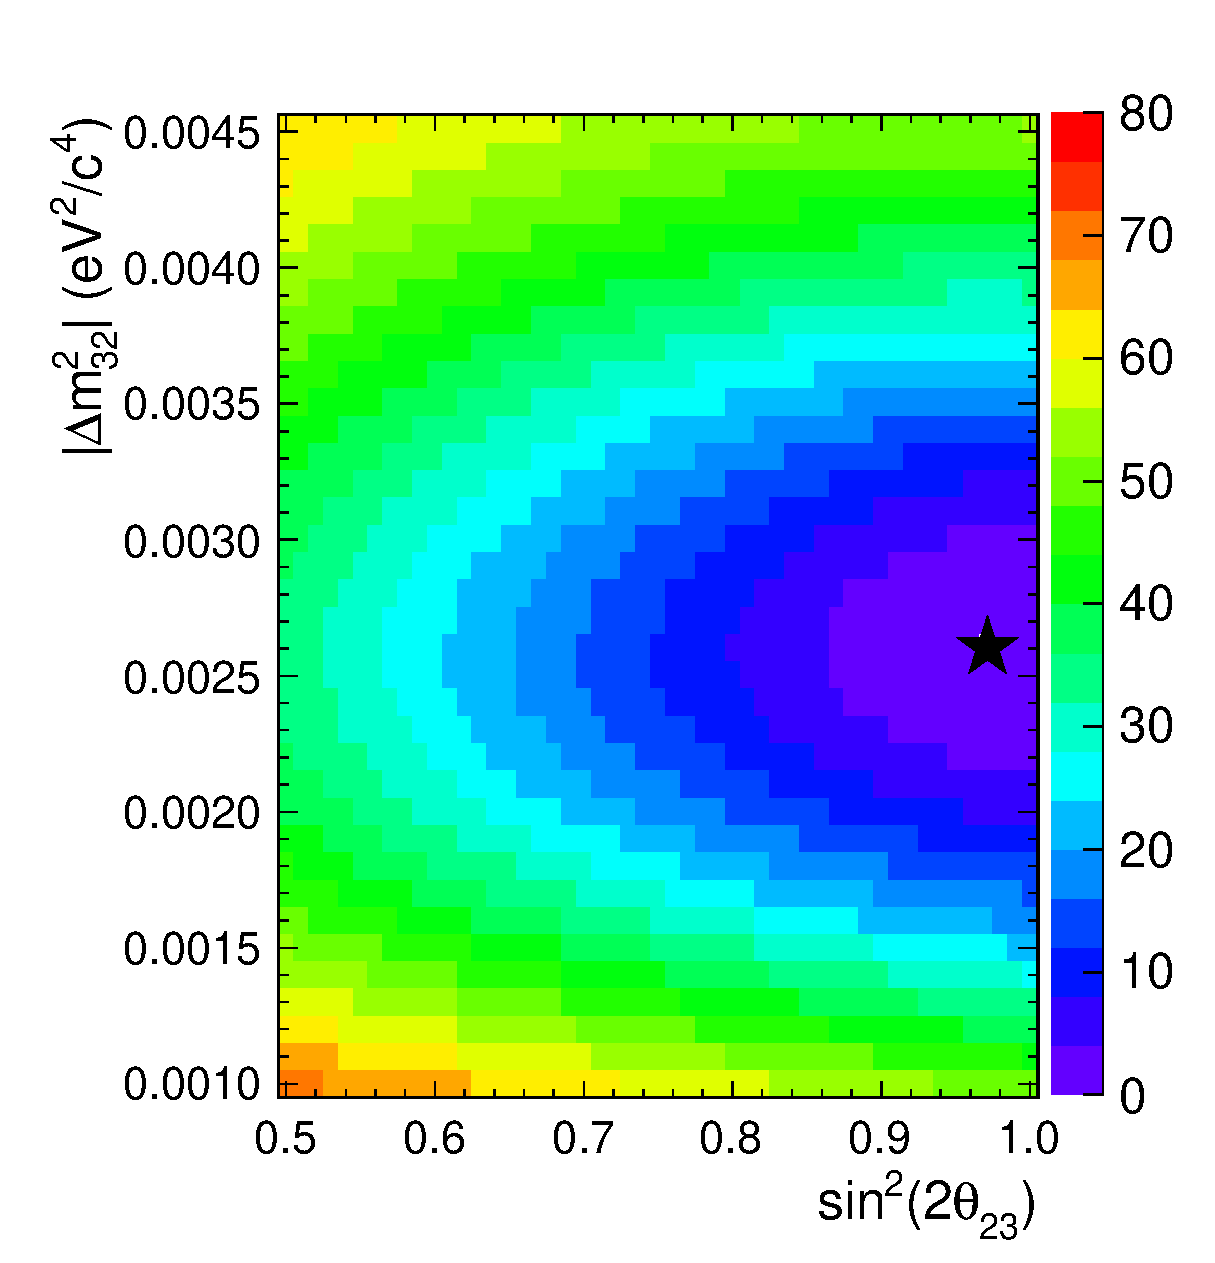
\includegraphics[width=18pc,height=19pc]{./images/fits/run1p2_genie_deltachisqsurf_zoom.eps}
\caption{
  $\Delta\chi^{2}$ surface for the 2-flavour disappearance fit to the combined 1.431$\times$10$^{20}$ POT Run1+2 dataset, 
  zoomed around the best-fit value (GENIE)
}
\label{fig:run1p2_genie_deltachisqsurf_zoom}
\end{minipage}
\hspace{0.06\linewidth}
\begin{minipage}[t]{0.47\linewidth}
\centering  
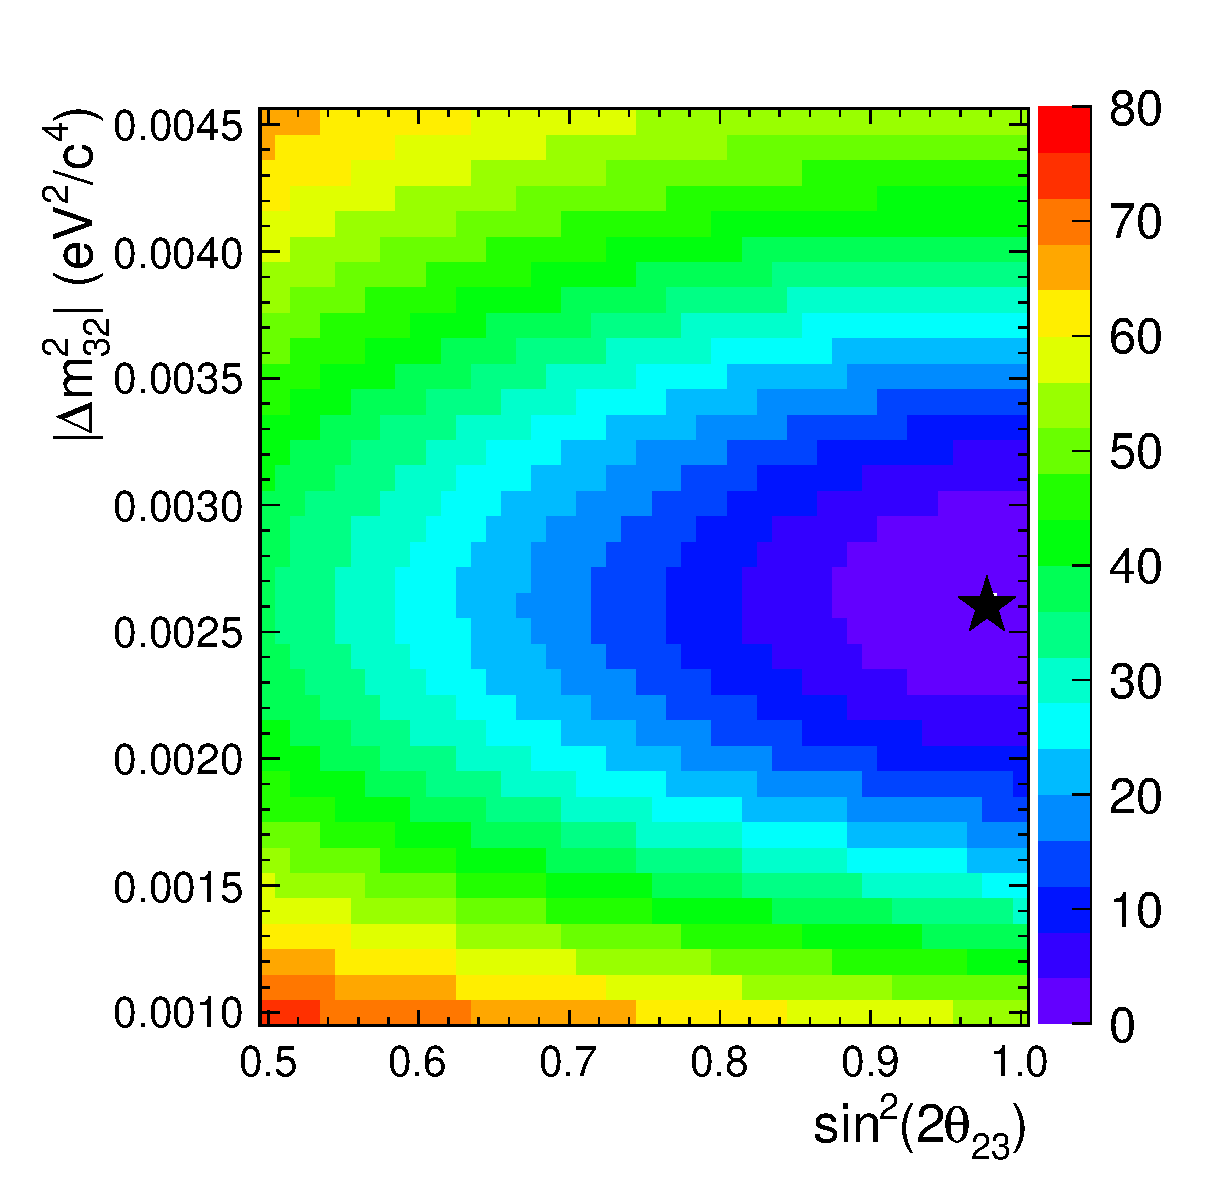
\includegraphics[width=18pc,height=19pc]{./images/fits/run1p2_neut_deltachisqsurf_zoom.eps}
\caption{
  $\Delta\chi^{2}$ surface for the 2-flavour disappearance fit to the combined 1.431$\times$10$^{20}$ POT Run1+2 dataset,
  zoomed around the best-fit value (NEUT)
}
\label{fig:run1p2_neut_deltachisqsurf_zoom}
\end{minipage}
\end{figure}

%
% Run1+2 marginalised delta chisq distributions
%

\begin{figure*}[htb]
\center
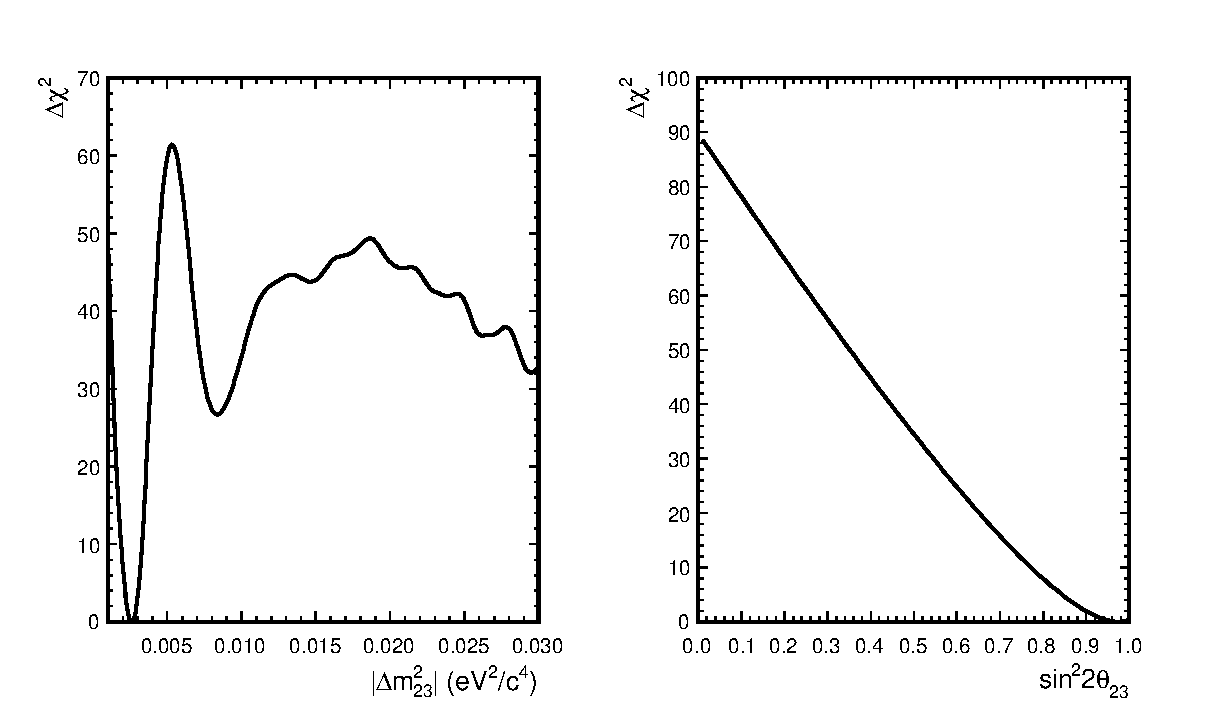
\includegraphics[width=34pc]{./images/fits/run1p2_genie_marginal_deltachisq_wide.eps}
\caption{
  Marginalised $\Delta\chi^{2}$ distributions from the 2-flavour $\nu_{\mu}$-disappearance fit 
  to the combined 1.431$\times$10$^{20}$ POT Run1+2 dataset (GENIE)
}
\label{fig:run1p2_genie_marginal_deltachisq_wide}
\end{figure*}

\begin{figure*}[htb]
\center
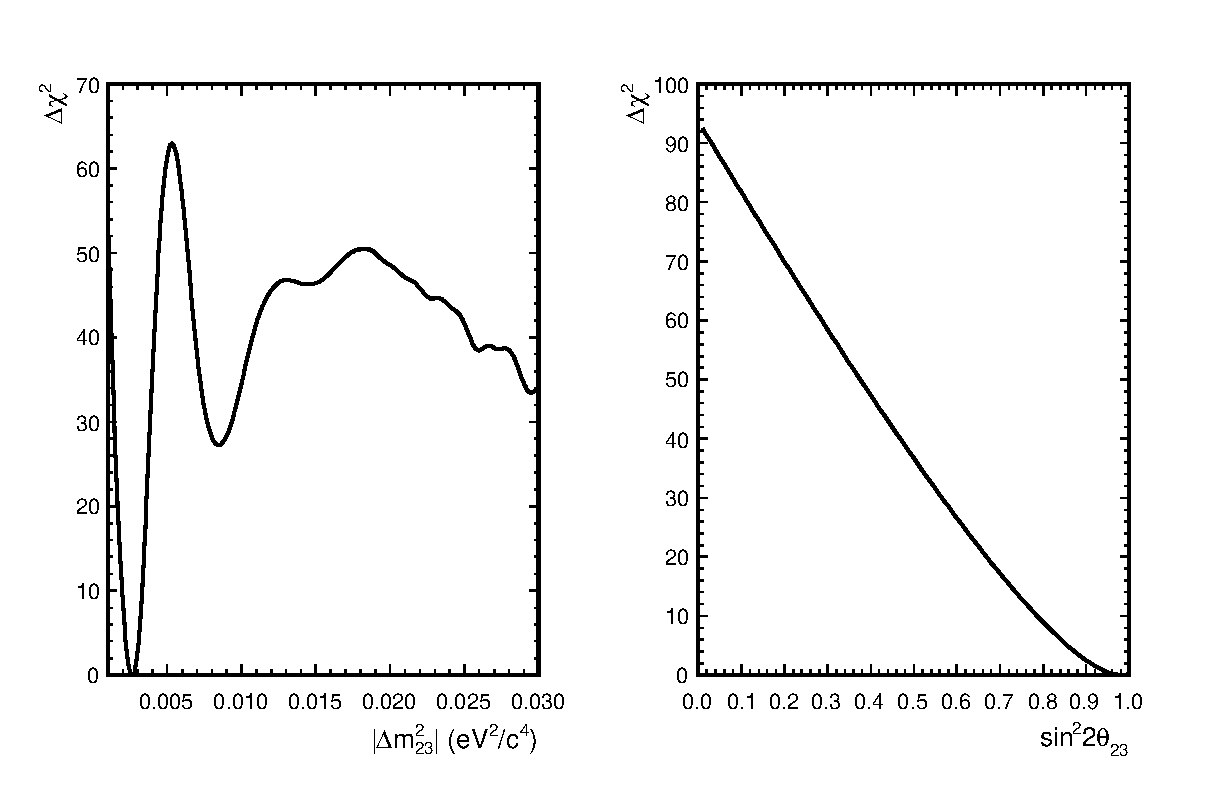
\includegraphics[width=34pc]{./images/fits/run1p2_neut_marginal_deltachisq_wide.eps}
\caption{
  Marginalised $\Delta\chi^{2}$ distributions from the 2-flavour $\nu_{\mu}$-disappearance fit 
  to the combined 1.431$\times$10$^{20}$ POT Run1+2 dataset (NEUT)
}
\label{fig:run1p2_neut_marginal_deltachisq_wide}
\end{figure*}

%
% Chisq and best-fit distributions for fits to 1.431E+20 POT toy MC expts generated with the MINOS-2011 params.
%

\begin{figure*}[ht]
\centering
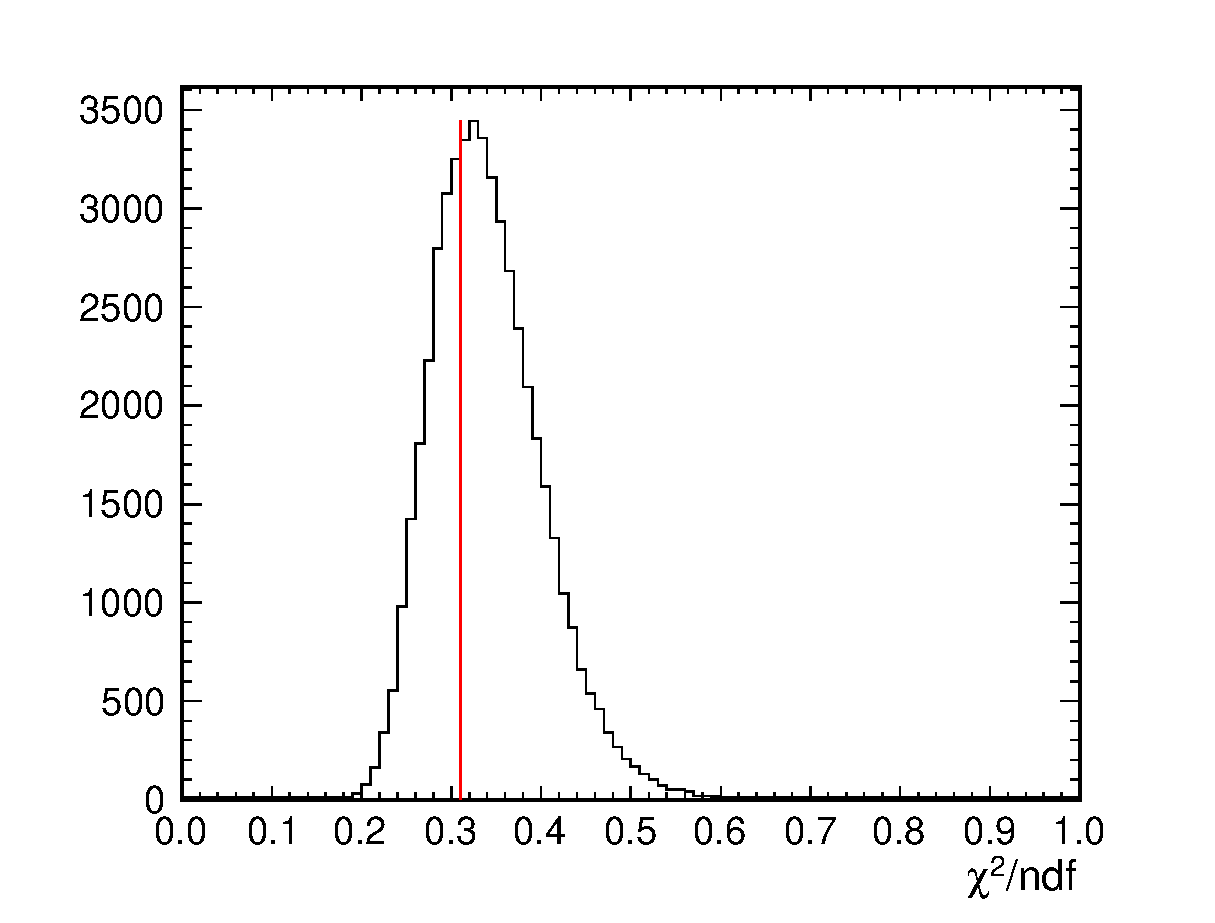
\includegraphics[height=21pc]{./images/fits/genie-minos11-run1p2-toymc-chisq-distribution.eps}
\caption{
  $chi^{2}/ndf$ distribution for fits to 1.431$\times$10$^{20}$ POT toy MC experiments 
  generated with $sin^{2}2\theta_{23}$ = 1.0 and $|\Delta m^{2}_{23}|$ = 2.32$\times10^{-3}$ $eV^{2}/c^{4}$.
  The $chi^{2}/ndf$ value for the fit to the Run1+2 dataset is also shown with a red line (GENIE).
}
\label{fig:genie-minos11-run1p2-toymc-chisq-distribution}
\end{figure*}

\begin{figure*}[ht]
\centering
\centering  
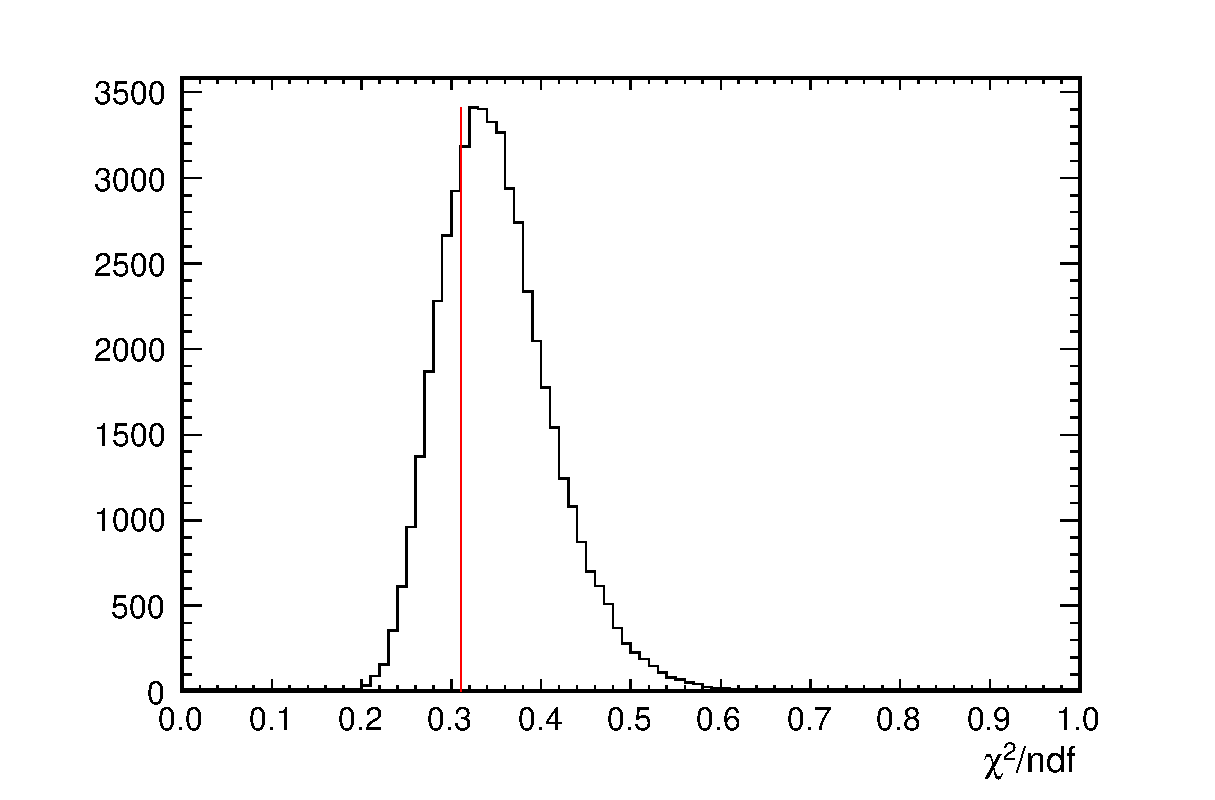
\includegraphics[height=21pc]{./images/fits/neut-minos11-run1p2-toymc-chisq-distribution.eps}
\caption{
  $chi^{2}/ndf$ distribution for fits to 1.431$\times$10$^{20}$ POT toy MC experiments 
  generated with $sin^{2}2\theta_{23}$ = 1.0 and $|\Delta m^{2}_{23}|$ = 2.32$\times10^{-3}$ $eV^{2}/c^{4}$.
  The $chi^{2}/ndf$ value for the fit to the Run1+2 dataset is also shown with a red line (NEUT).
}
\label{fig:neut-minos11-run1p2-toymc-chisq-distribution}
\end{figure*}


%\begin{figure}[ht]
%\begin{minipage}[t]{0.47\linewidth}
%\centering
%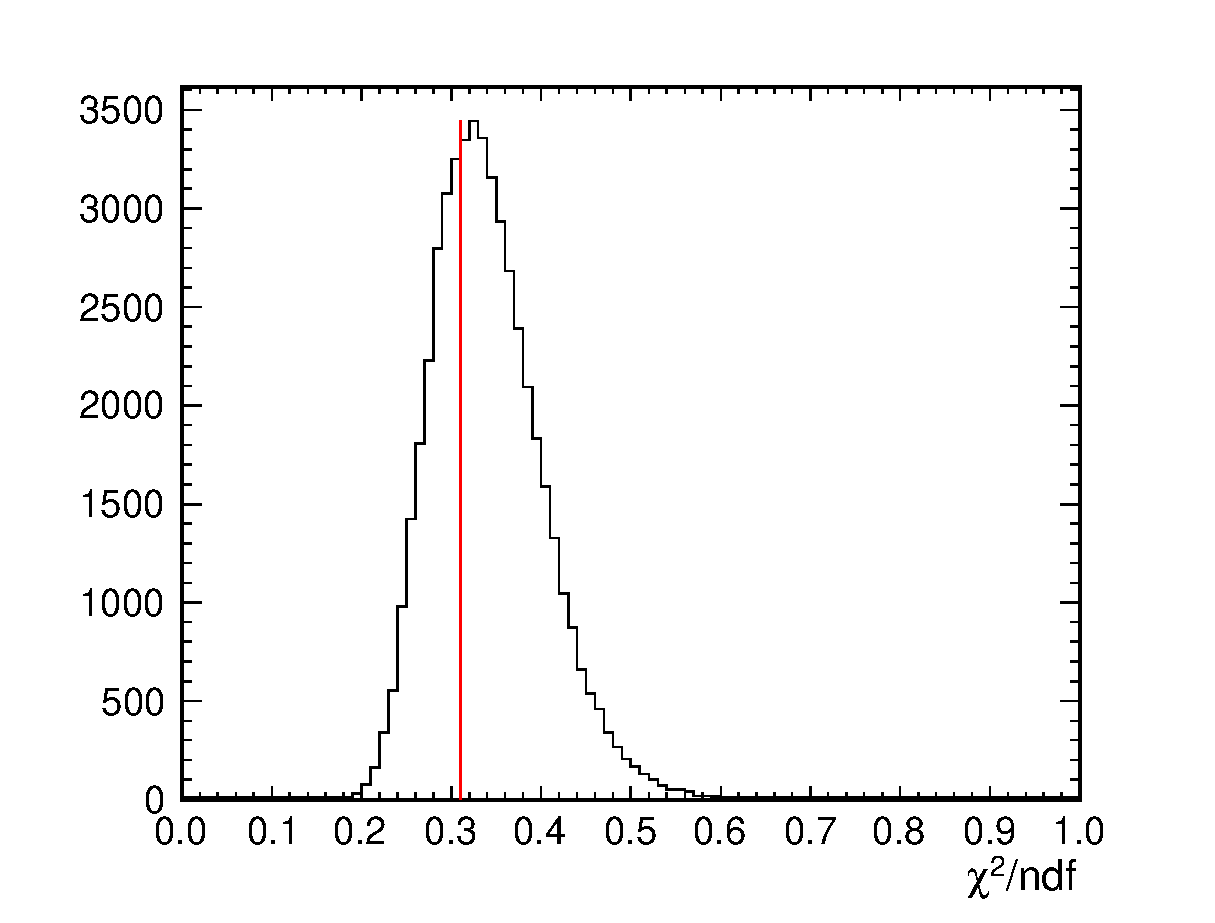
\includegraphics[width=18pc,height=19pc]{./images/fits/genie-minos11-run1p2-toymc-chisq-distribution.eps}
%\caption{
%  $chi^{2}/ndf$ distribution for fits to 1.431$\times$10$^{20}$ POT toy MC experiments 
%  generated with $sin^{2}2\theta_{23}$ = 1.0 and $|\Delta m^{2}_{23}|$ = 2.32$\times10^{-3}$ $eV^{2}/c^{4}$.
%  The $chi^{2}/ndf$ value for the fit to the Run1+2 dataset is also shown with a red line (GENIE).
%}
%\label{fig:genie-minos11-run1p2-toymc-chisq-distribution}
%\end{minipage}
%\hspace{0.06\linewidth}
%\begin{minipage}[t]{0.47\linewidth}
%\centering  
%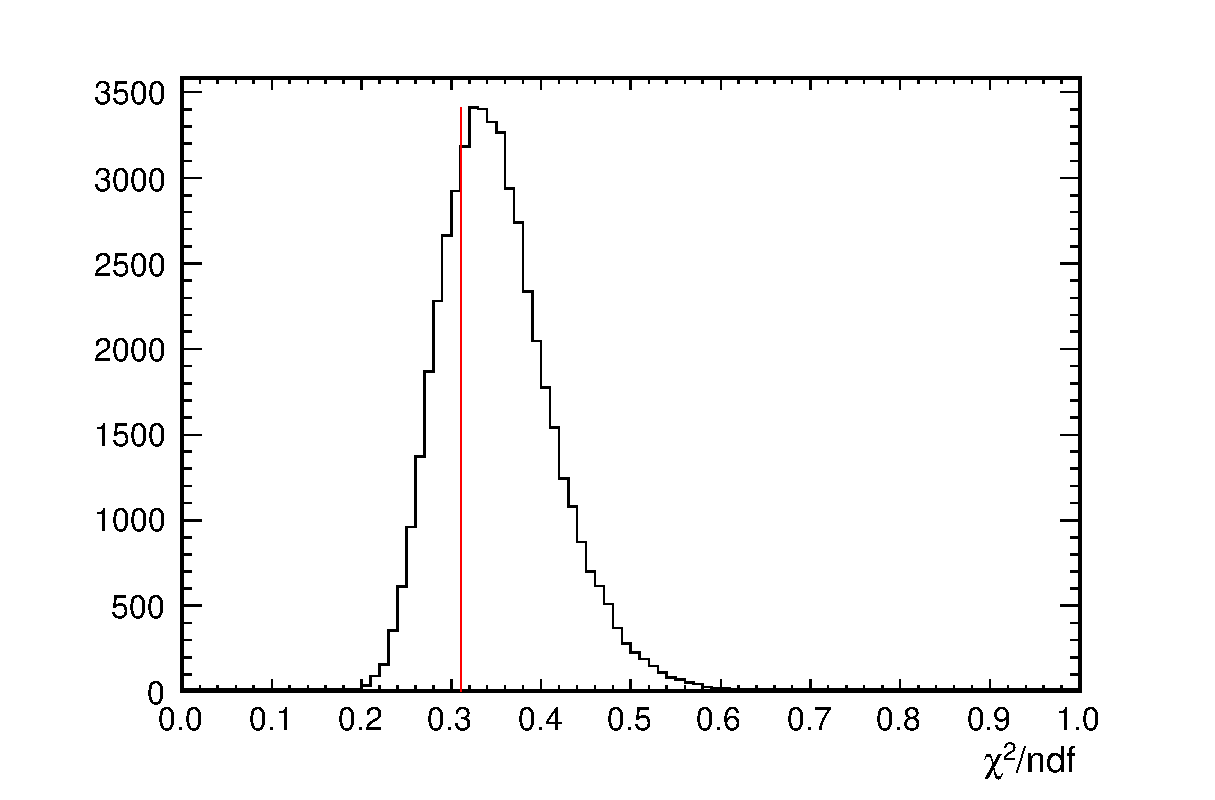
\includegraphics[width=18pc,height=19pc]{./images/fits/neut-minos11-run1p2-toymc-chisq-distribution.eps}
%\caption{
%  $chi^{2}/ndf$ distribution for fits to 1.431$\times$10$^{20}$ POT toy MC experiments 
%  generated with $sin^{2}2\theta_{23}$ = 1.0 and $|\Delta m^{2}_{23}|$ = 2.32$\times10^{-3}$ $eV^{2}/c^{4}$.
%  The $chi^{2}/ndf$ value for the fit to the Run1+2 dataset is also shown with a red line (NEUT).
%}
%\label{fig:neut-minos11-run1p2-toymc-chisq-distribution}
%\end{minipage}
%\end{figure}


\begin{figure*}[htb]
\center
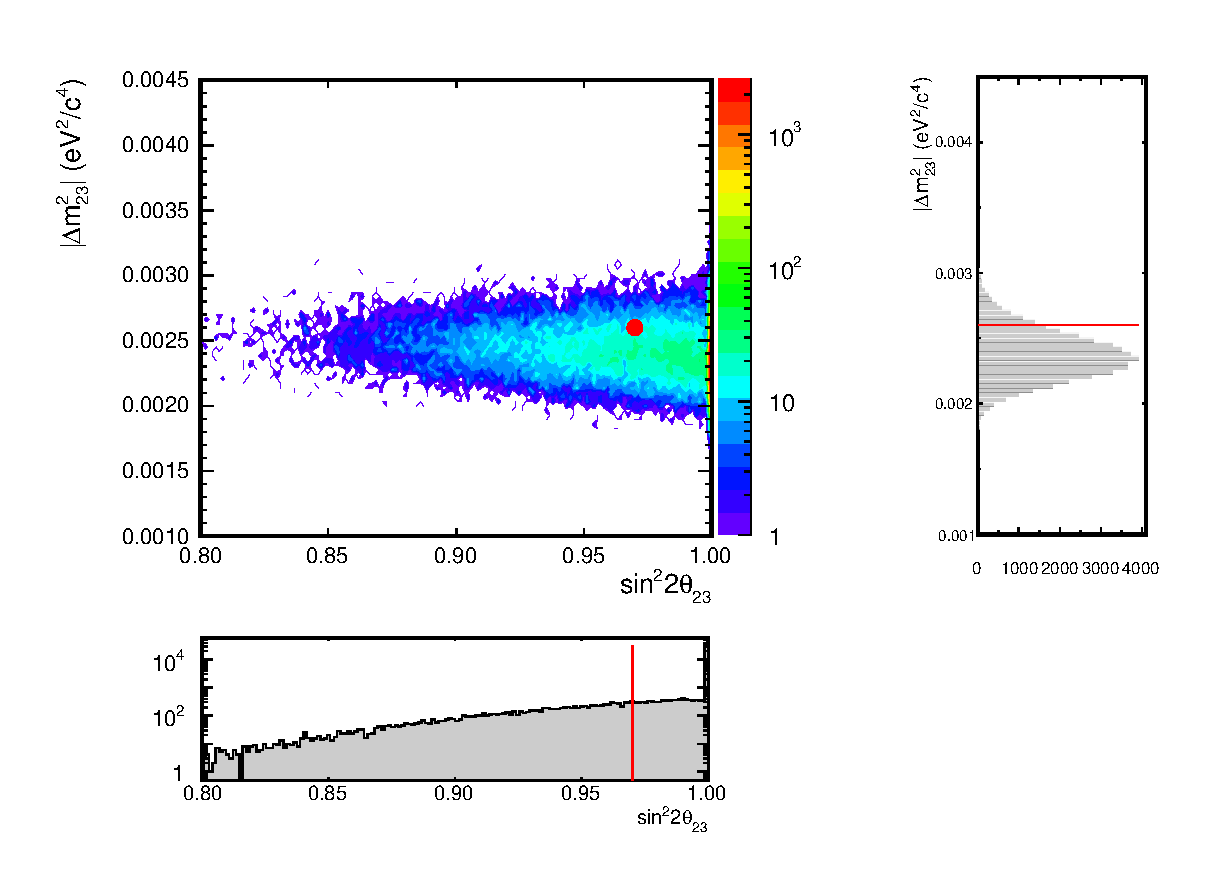
\includegraphics[width=35pc]{./images/fits/genie-minos11-run1p2-toymc-bestfitparam-distributions.eps}
\caption{
  Best-fit parameter distributions from 2-flavour $\nu_{\mu}$-disappearance 
  fits to 1.431$\times$10$^{20}$ POT toy MC experiments 
  generated with $sin^{2}2\theta_{23}$ = 1.0 and $|\Delta m^{2}_{23}|$ = 2.32$\times10^{-3}$ $eV^{2}/c^{4}$.
  The best-fit values for the fit to the Run1+2 dataset are also shown with a red marker and red lines (GENIE).
}
\label{fig:genie-minos11-run1p2-toymc-bestfitparam-distributions}
\end{figure*}

\begin{figure*}[htb]
\center
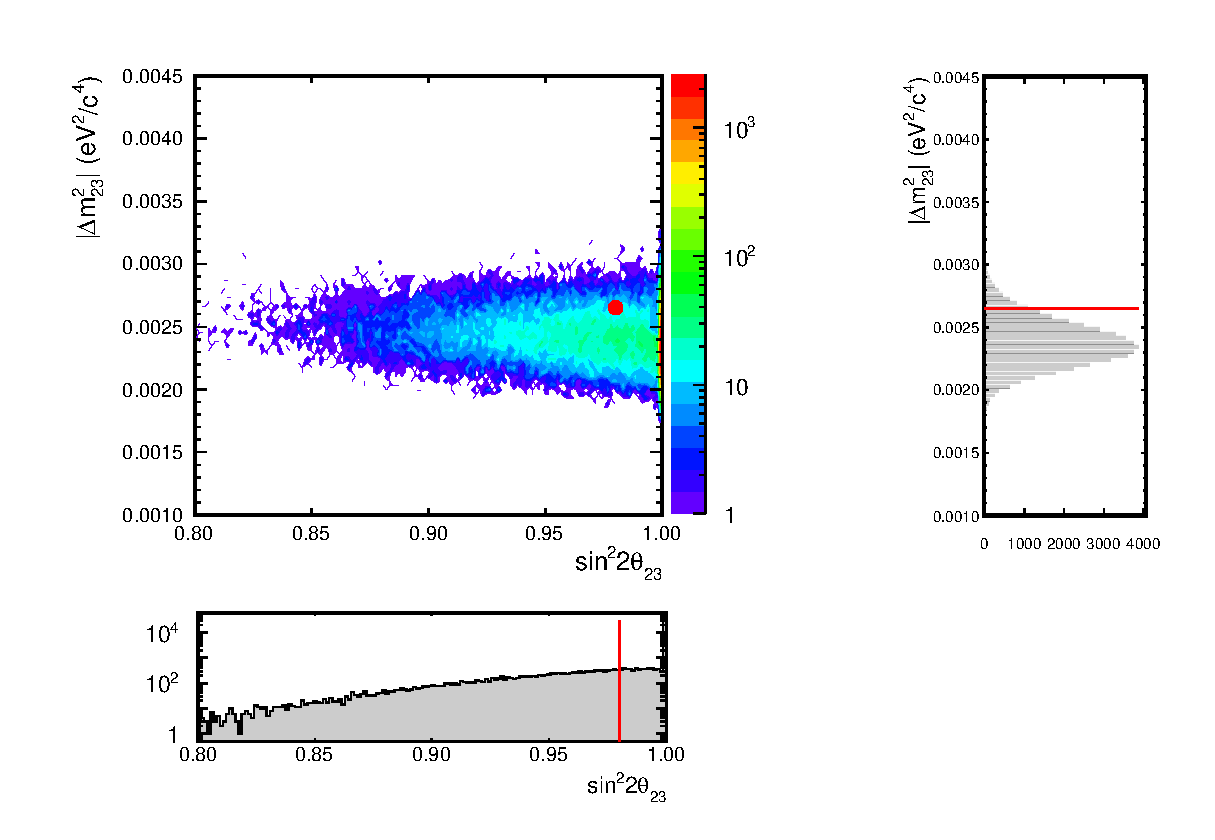
\includegraphics[width=35pc]{./images/fits/neut-minos11-run1p2-toymc-bestfitparam-distributions.eps}
\caption{
  Best-fit parameter distributions from 2-flavour $\nu_{\mu}$-disappearance 
  fits to 1.431$\times$10$^{20}$ POT toy MC experiments 
  generated with $sin^{2}2\theta_{23}$ = 1.0 and $|\Delta m^{2}_{23}|$ = 2.32$\times10^{-3}$ $eV^{2}/c^{4}$.
  The best-fit values for the fit to the Run1+2 dataset are also shown with a red marker and red lines (NEUT).
}
\label{fig:neut-minos11-run1p2-toymc-bestfitparam-distributions}
\end{figure*}

\clearpage

%
% Run1 fit data/best-fit distribution (variable binning + CCQE/other)
%

\begin{figure*}[htb]
\center
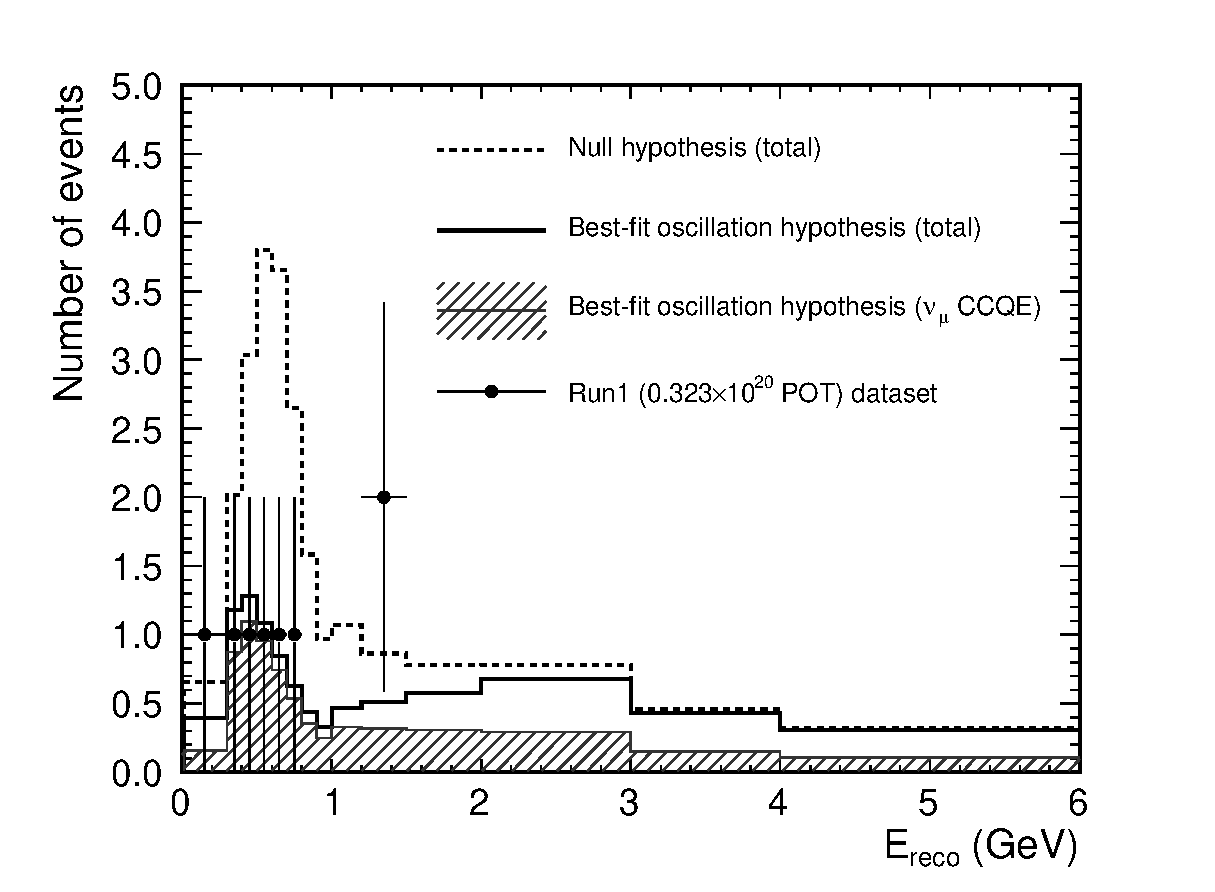
\includegraphics[height=19pc]{./images/fits/run1_genie_bestfit_spectrum_rebin_modes.eps}
\caption{
  Reconstructed neutrino energy distribution of the 8 single $\mu$-like ring events of the
  0.323$\times$10$^{20}$ POT Run1 dataset (points) and GENIE best-fit SuperK prediction (solid line).
  The best-fit oscillation parameters are
  $|\Delta m^{2}_{23}|$ = 2.77$\times$10$^{-3}$ $eV^{2}/c^{4}$ and $sin^{2}2\theta_{23}$ = 0.81
  (local minimum in first oscillation maximum region).
  The dotted line shows the GENIE prediction without oscillations.
  The distributions are not shown with 50 MeV bins as used in the oscillation fit,
  but with fewer, variable-size bins for illustration purposes.
}
\label{fig:run1_spectrum_and_data_genie_rebin_modes}
\end{figure*}

\begin{figure*}[htb]
\center
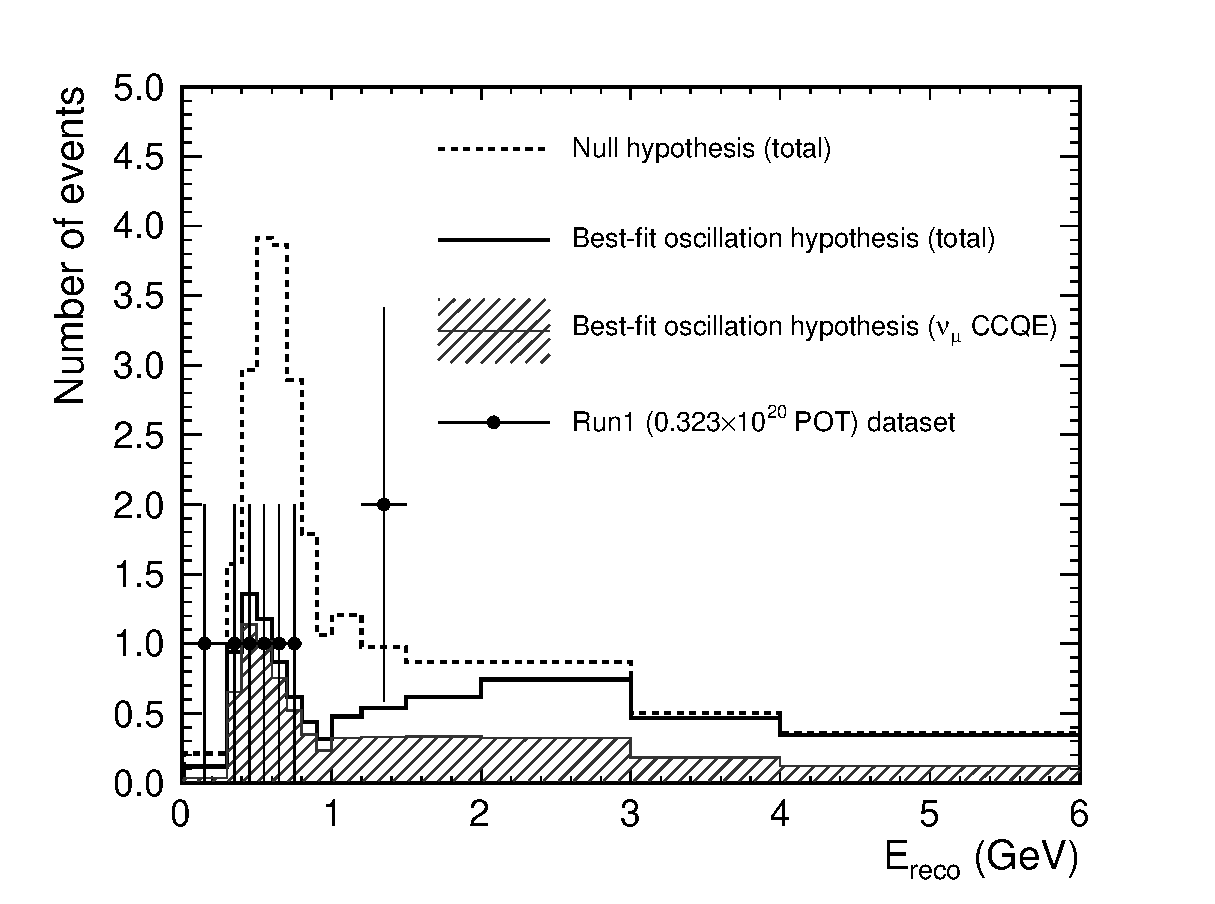
\includegraphics[height=19pc]{./images/fits/run1_neut_bestfit_spectrum_rebin_modes.eps}
\caption{
  Reconstructed neutrino energy distribution of the 8 single $\mu$-like ring events of the
  0.323$\times$10$^{20}$ POT Run1 dataset (points) and NEUT best-fit SuperK prediction (solid line).
  The best-fit oscillation parameters are
  $|\Delta m^{2}_{23}|$ = 2.88$\times$10$^{-3}$ $eV^{2}/c^{4}$ and $sin^{2}2\theta_{23}$ = 0.84
  (local minimum in first oscillation maximum region).
  The dotted line shows the NEUT prediction without oscillations.
  The distributions are not shown with 50 MeV bins as used in the oscillation fit,
  but with fewer, variable-size bins for illustration purposes.
}
\label{fig:run1_spectrum_and_data_neut_rebin_modes}
\end{figure*}


%
% Run2 fit data/best-fit distribution (variable binning + CCQE/other)
%

\begin{figure*}[htb]
\center
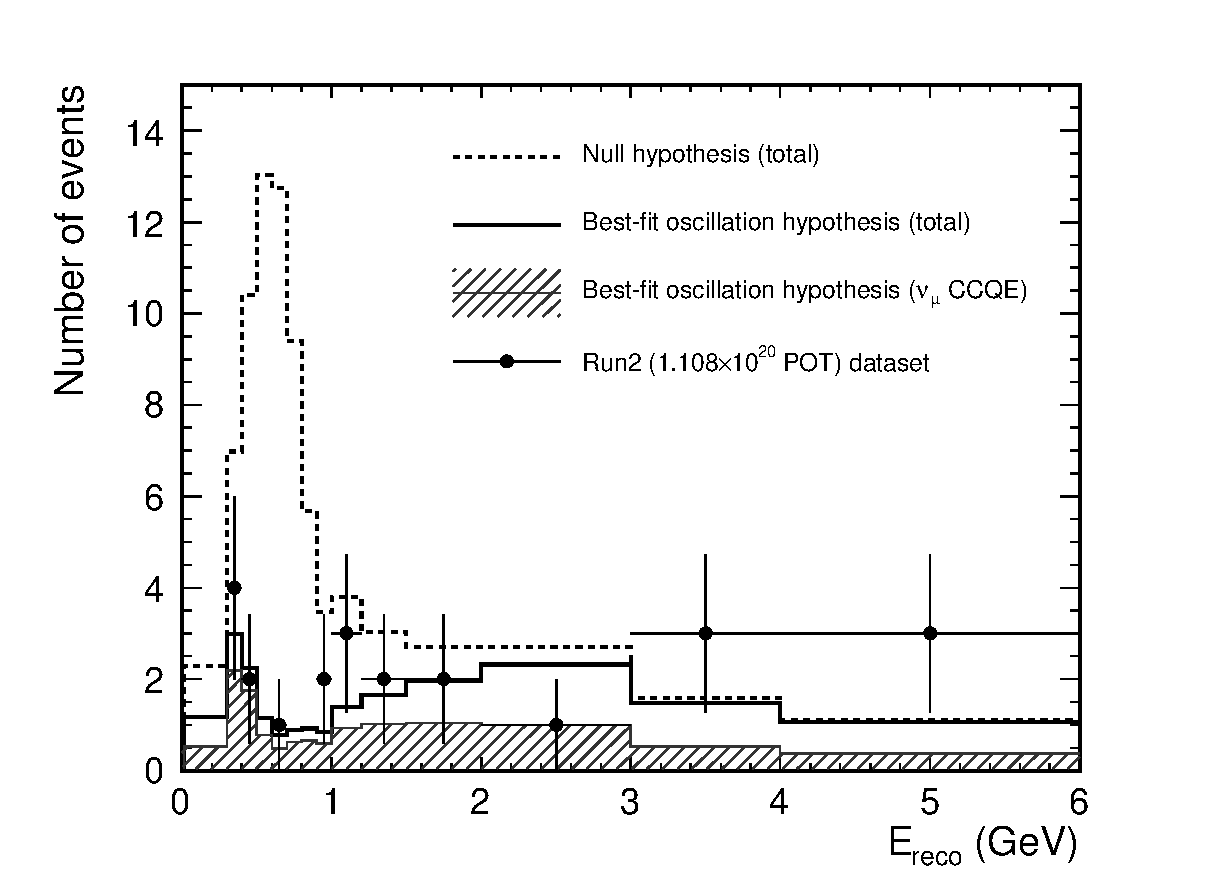
\includegraphics[width=32pc]{./images/fits/run2_genie_bestfit_spectrum_rebin_modes.eps}
\caption{
  Reconstructed neutrino energy distribution of the 23 single $\mu$-like ring events of the
  1.108$\times$10$^{20}$ POT Run2 dataset (points) and GENIE best-fit SuperK prediction (solid line).
  The best-fit oscillation parameters are
  $|\Delta m^{2}_{23}|$ = 2.59$\times$10$^{-3}$ $eV^{2}/c^{4}$ and $sin^{2}2\theta_{23}$ = 1.00.
  The dotted line shows the GENIE prediction without oscillations.
  The distributions are not shown with 50 MeV bins as used in the oscillation fit,
  but with fewer, variable-size bins for illustration purposes.
}
\label{fig:run2_spectrum_and_data_genie_rebin_modes}
\end{figure*}

\begin{figure*}[htb]
\center
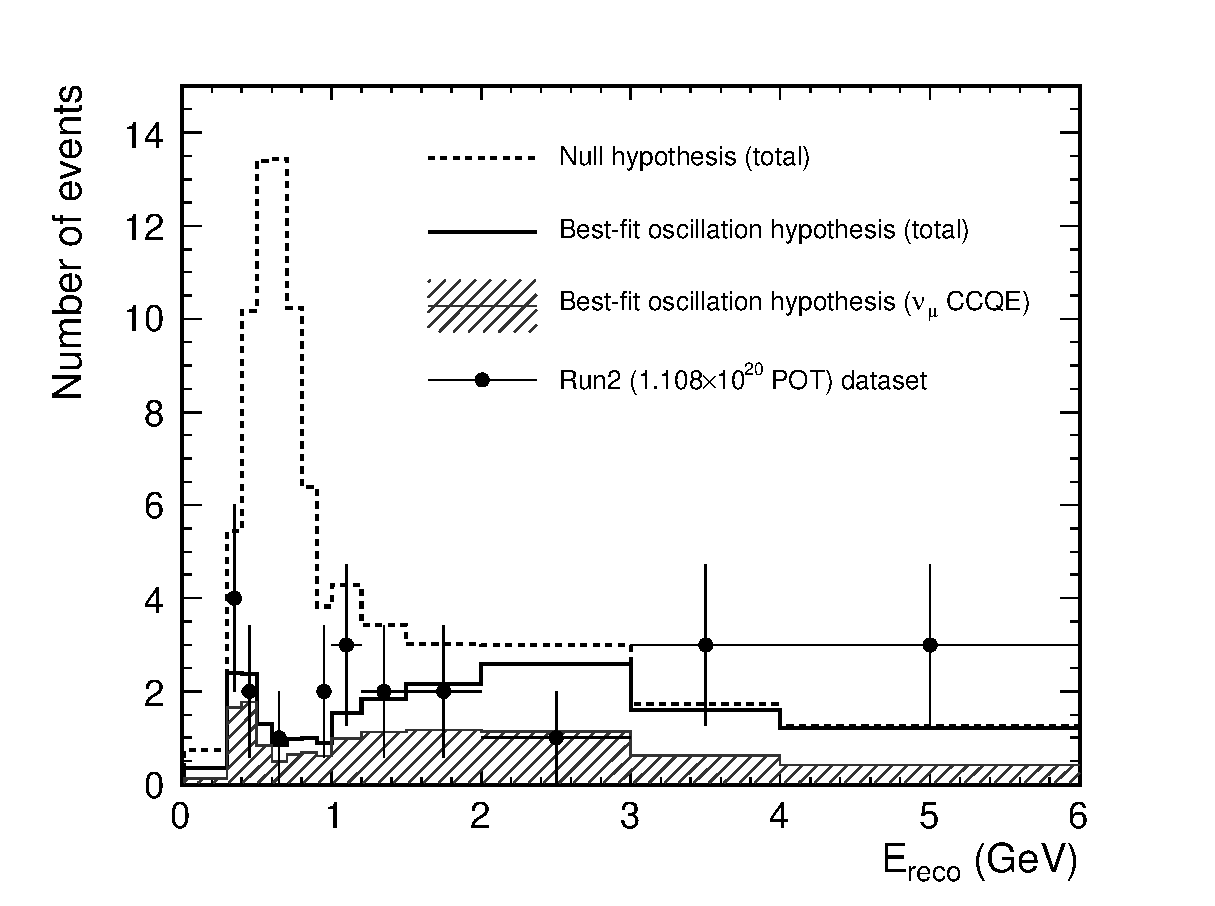
\includegraphics[width=32pc]{./images/fits/run2_neut_bestfit_spectrum_rebin_modes.eps}
\caption{
  Reconstructed neutrino energy distribution of the 23 single $\mu$-like ring events of the
  1.108$\times$10$^{20}$ POT Run2 dataset (points) and NEUT best-fit SuperK prediction (solid line).
  The best-fit oscillation parameters are
  $|\Delta m^{2}_{23}|$ = 2.62$\times$10$^{-3}$ $eV^{2}/c^{4}$ and $sin^{2}2\theta_{23}$ = 1.00.
  The dotted line shows the NEUT prediction without oscillations.
  The distributions are not shown with 50 MeV bins as used in the oscillation fit,
  but with fewer, variable-size bins for illustration purposes.
}
\label{fig:run2_spectrum_and_data_neut_rebin_modes}
\end{figure*}


%
% Run1, Run2 and Run1+2 marginalised chisq distributions
%

% dmsq (restricted)
\begin{figure}[ht]
\begin{minipage}[t]{0.47\linewidth}
\centering
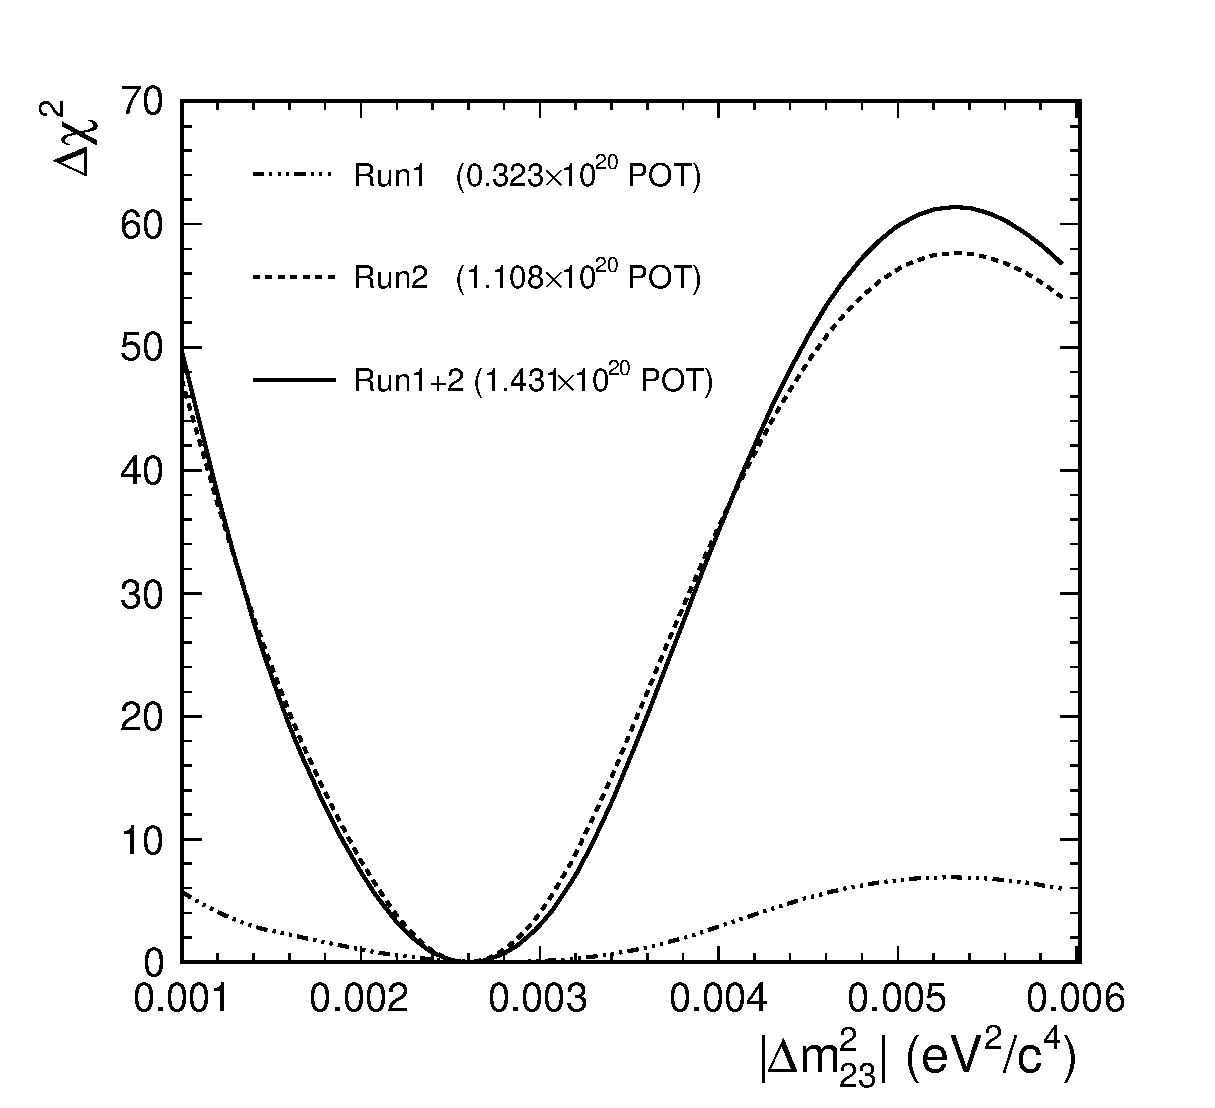
\includegraphics[width=18pc,height=19pc]{./images/fits/genie_marginal_deltachisq_dmsq_narrow_3datasets.eps}
\caption{
  The marginalised $\Delta\chi^{2}$ distributions as a function of $|\Delta m^{2}_{23}|$ from the 2-flavour
  $\nu_{\mu}$-disappearance fits to the Run1, Run2 and Run1+2 datasets (GENIE).
  All fits were performed in the restricted $|\Delta m^{2}_{23}|$ range from
  1$\times$10$^{-3}$ $eV^{2}/c^{4}$ to 6$\times$10$^{-3}$ $eV^{2}/c^{4}$.
}
\label{fig:genie_deltachisq_dmsq_narrow_3datasets}
\end{minipage}
\hspace{0.06\linewidth}
\begin{minipage}[t]{0.47\linewidth}
\centering  
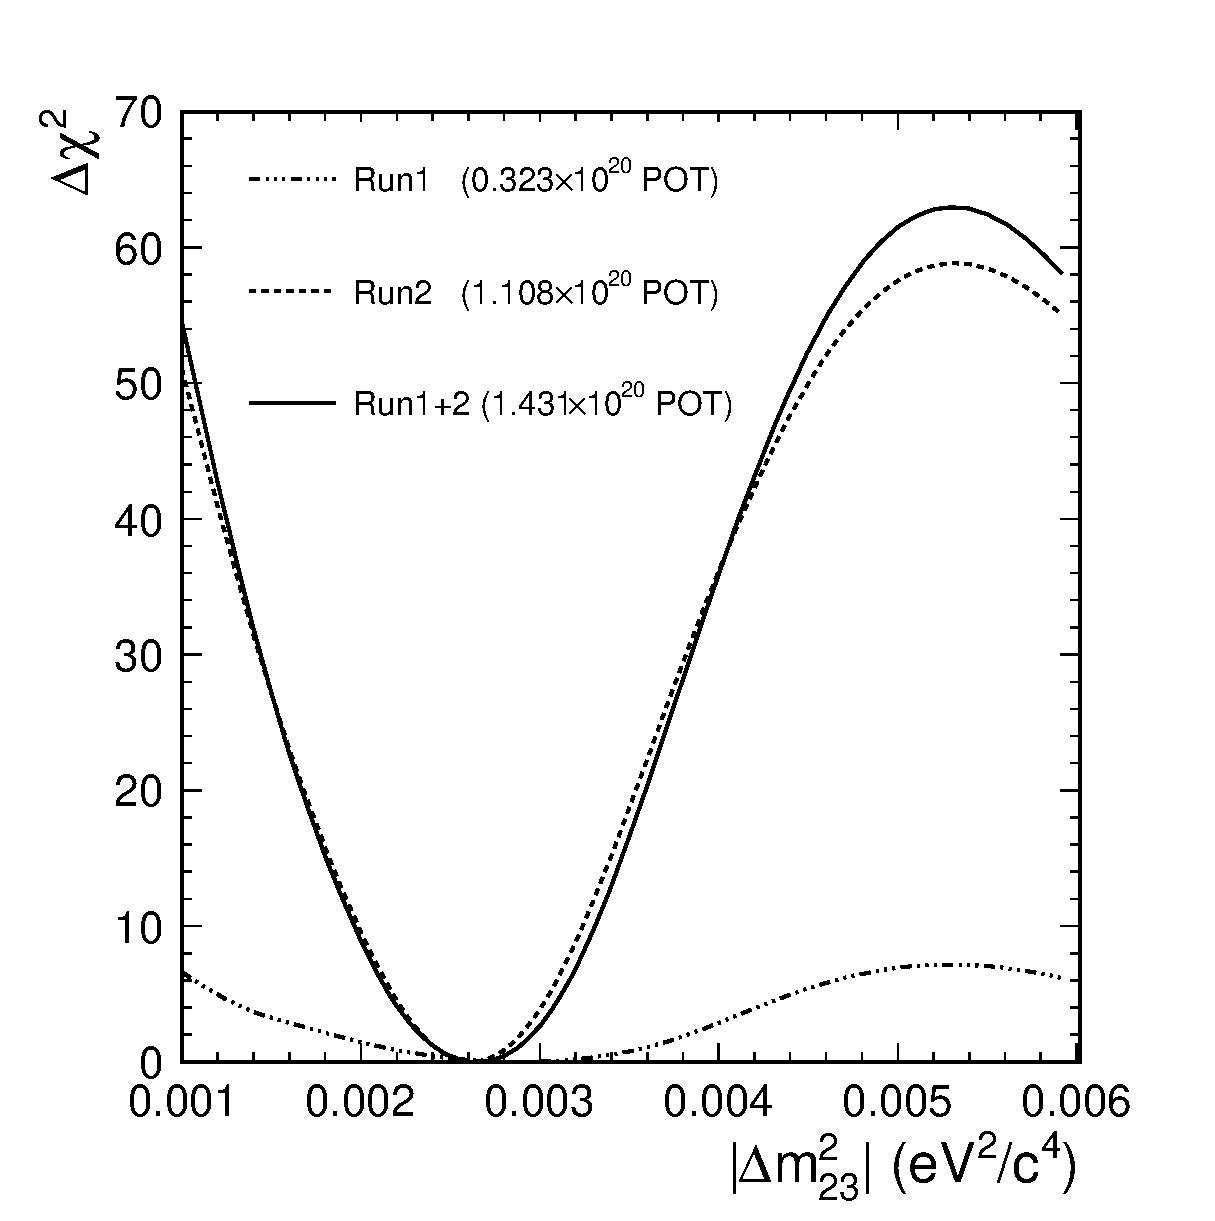
\includegraphics[width=18pc,height=19pc]{./images/fits/neut_marginal_deltachisq_dmsq_narrow_3datasets.eps}
\caption{
  The marginalised $\Delta\chi^{2}$ distributions as a function of $|\Delta m^{2}_{23}|$ from the 2-flavour
  $\nu_{\mu}$-disappearance fits to the Run1, Run2 and Run1+2 datasets (NEUT).
  All fits were performed in the restricted $|\Delta m^{2}_{23}|$ range from
  1$\times$10$^{-3}$ $eV^{2}/c^{4}$ to 6$\times$10$^{-3}$ $eV^{2}/c^{4}$.
}
\label{fig:neut_deltachisq_dmsq_narrow_3datasets}
\end{minipage}
\end{figure}

% dmsq (wide)
\begin{figure}[ht]
\begin{minipage}[t]{0.47\linewidth}
\centering
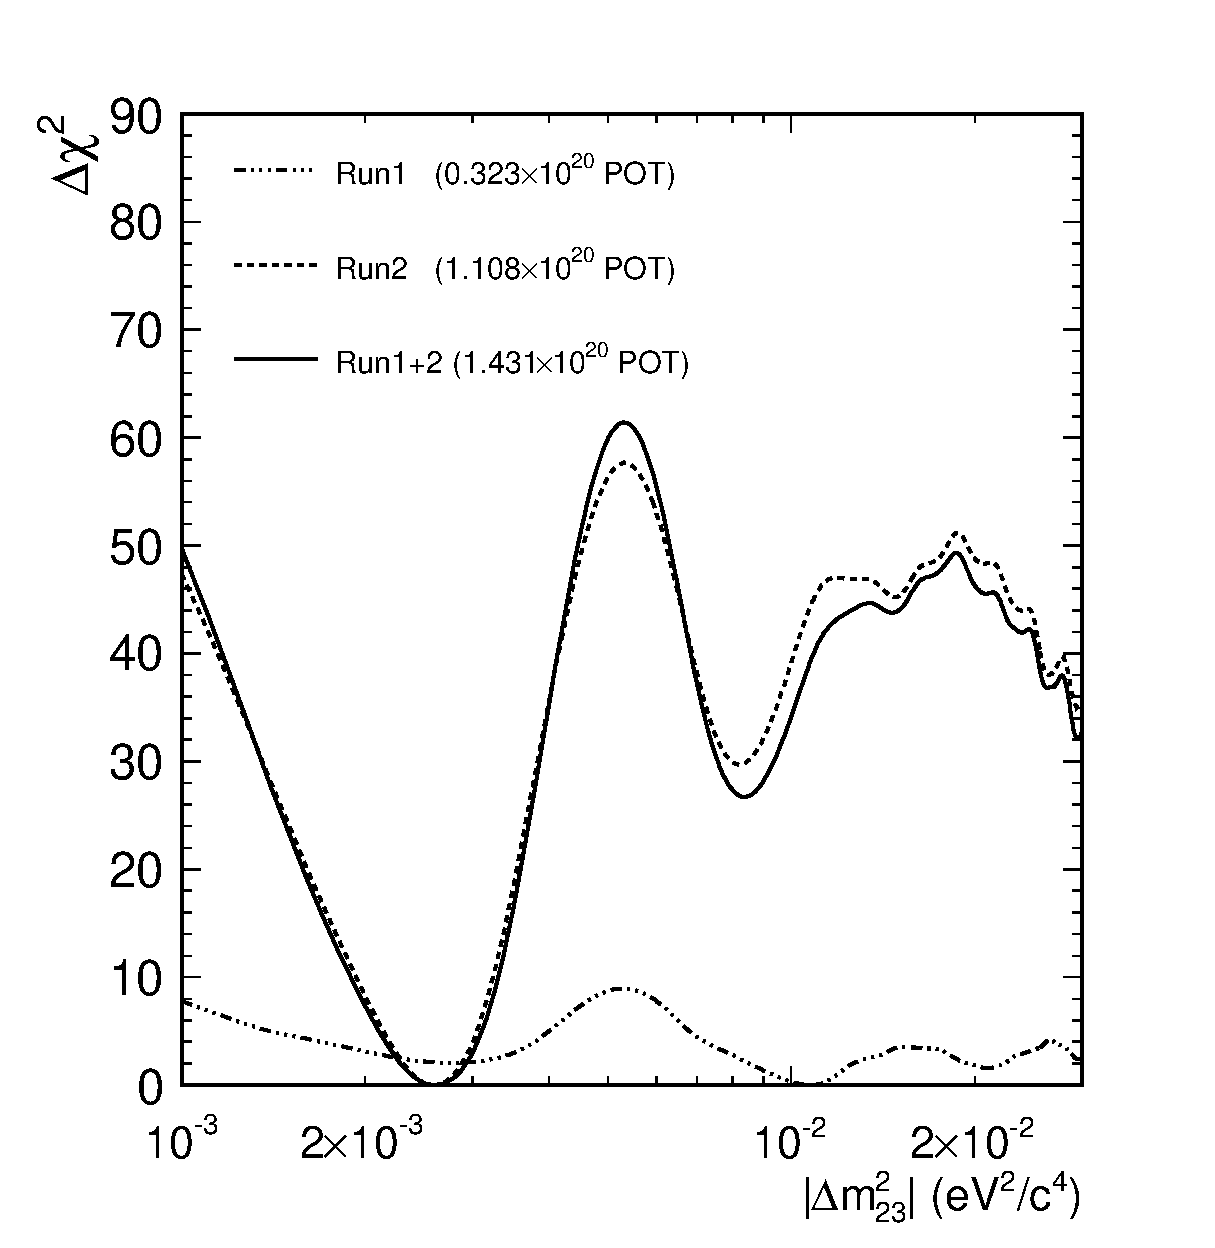
\includegraphics[width=18pc,height=19pc]{./images/fits/genie_marginal_deltachisq_dmsq_wide_3datasets.eps}
\caption{
  The marginalised $\Delta\chi^{2}$ distributions as a function of $|\Delta m^{2}_{23}|$ from the 2-flavour
  $\nu_{\mu}$-disappearance fits to the Run1, Run2 and Run1+2 datasets (GENIE).
  All fits were performed in the extended $|\Delta m^{2}_{23}|$ range from 
  1$\times$10$^{-3}$ $eV^{2}/c^{4}$ to 30$\times$10$^{-3}$ $eV^{2}/c^{4}$.
}
\label{fig:genie_deltachisq_dmsq_wide_3datasets}
\end{minipage}
\hspace{0.06\linewidth}
\begin{minipage}[t]{0.47\linewidth}
\centering  
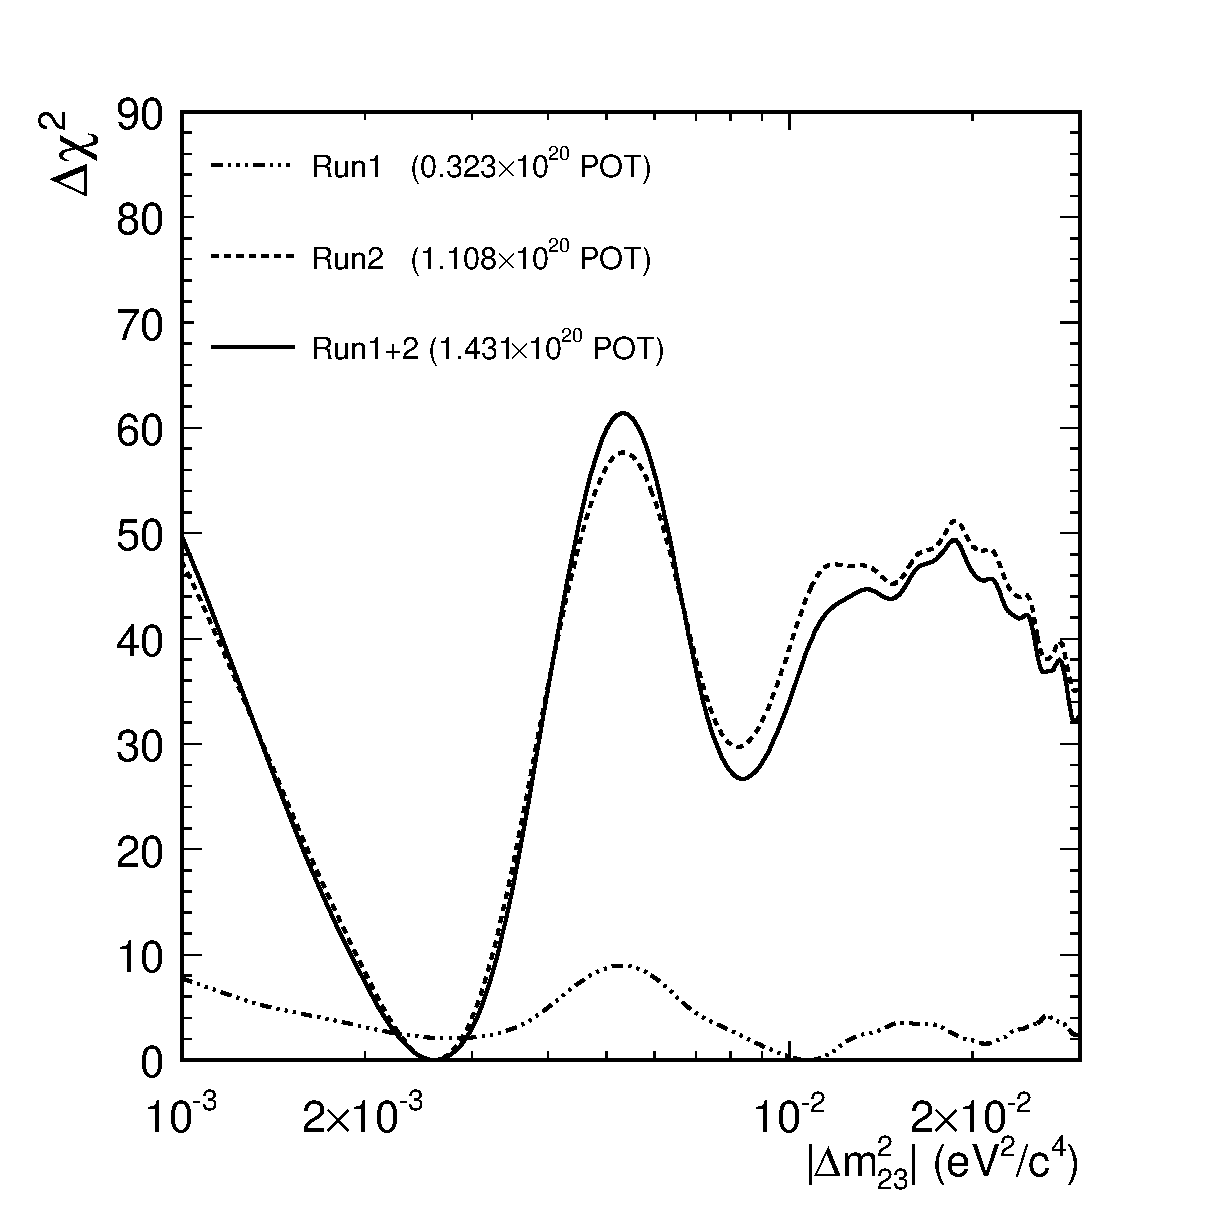
\includegraphics[width=18pc,height=19pc]{./images/fits/neut_marginal_deltachisq_dmsq_wide_3datasets.eps}
\caption{
  The marginalised $\Delta\chi^{2}$ distributions as a function of $|\Delta m^{2}_{23}|$ from the 2-flavour
  $\nu_{\mu}$-disappearance fits to the Run1, Run2 and Run1+2 datasets (NEUT).
  All fits were performed in the extended $|\Delta m^{2}_{23}|$ range from 
  1$\times$10$^{-3}$ $eV^{2}/c^{4}$ to 30$\times$10$^{-3}$ $eV^{2}/c^{4}$.
}
\label{fig:neut_deltachisq_dmsq_wide_3datasets}
\end{minipage}
\end{figure}


% sinsq2theta23
\begin{figure}[ht]
\begin{minipage}[t]{0.47\linewidth}
\centering
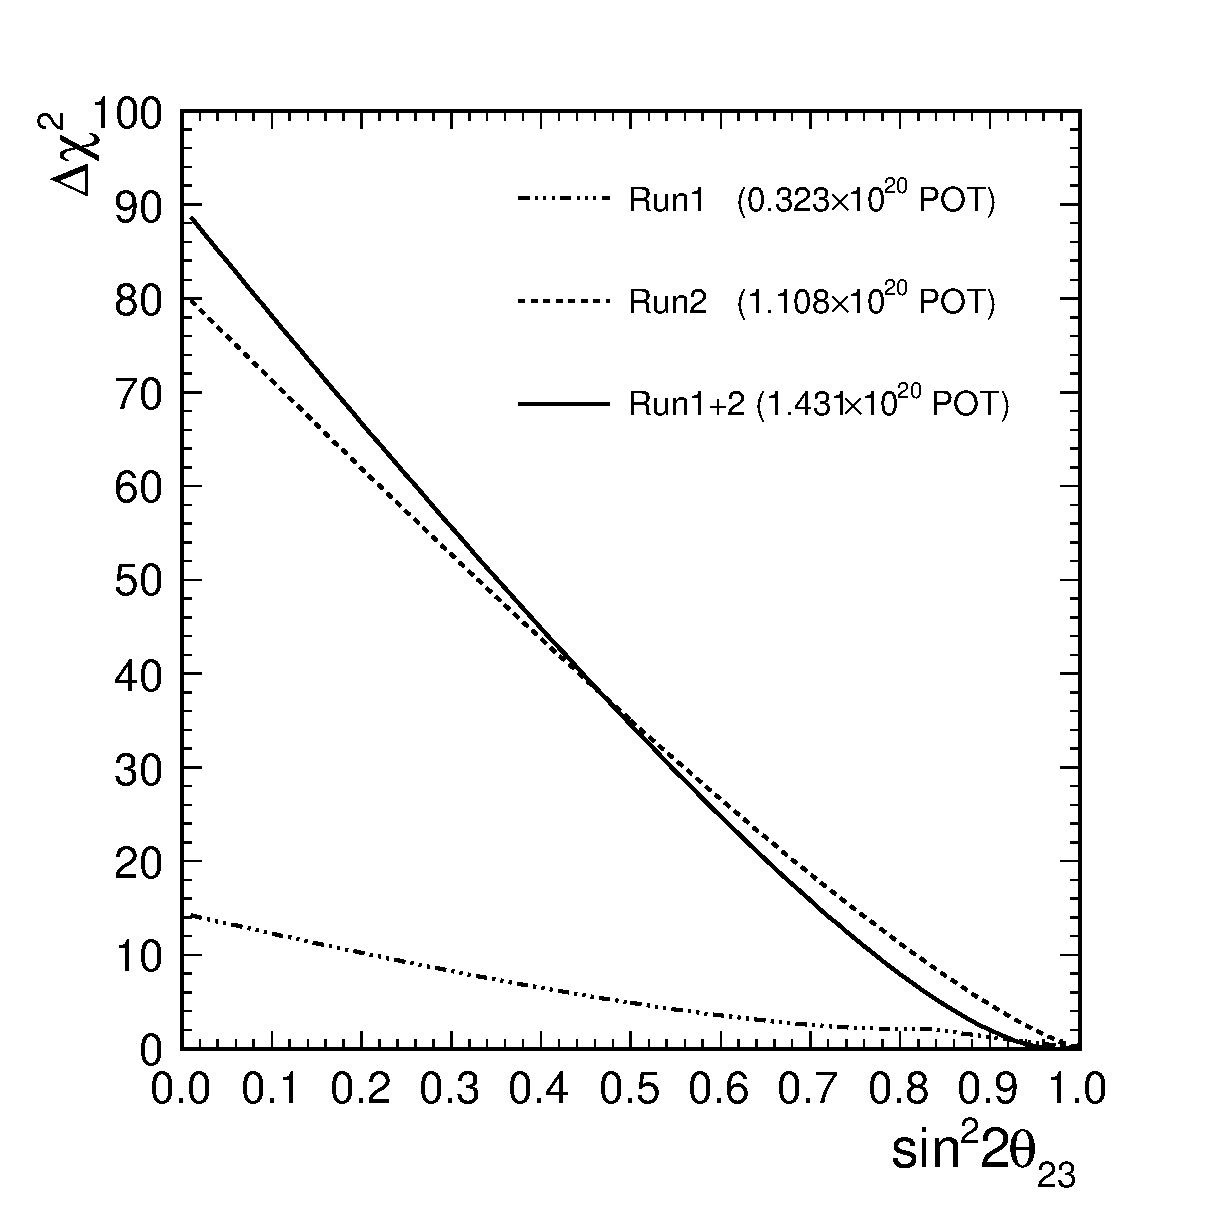
\includegraphics[width=18pc,height=19pc]{./images/fits/genie_marginal_deltachisq_sinsq2theta_3datasets.eps}
\caption{
  The marginalised $\Delta\chi^{2}$ distributions as a function of $sin^{2}2\theta_{23}$ from the 2-flavour
  $\nu_{\mu}$-disappearance fits to the Run1, Run2 and Run1+2 datasets (GENIE).
  All fits were performed in the restricted $|\Delta m^{2}_{23}|$ range from 
  1$\times$10$^{-3}$ $eV^{2}/c^{4}$ to 6$\times$10$^{-3}$ $eV^{2}/c^{4}$.
}
\label{fig:genie_deltachisq_sinsq2theta_3datasets}
\end{minipage}
\hspace{0.06\linewidth}
\begin{minipage}[t]{0.47\linewidth}
\centering  
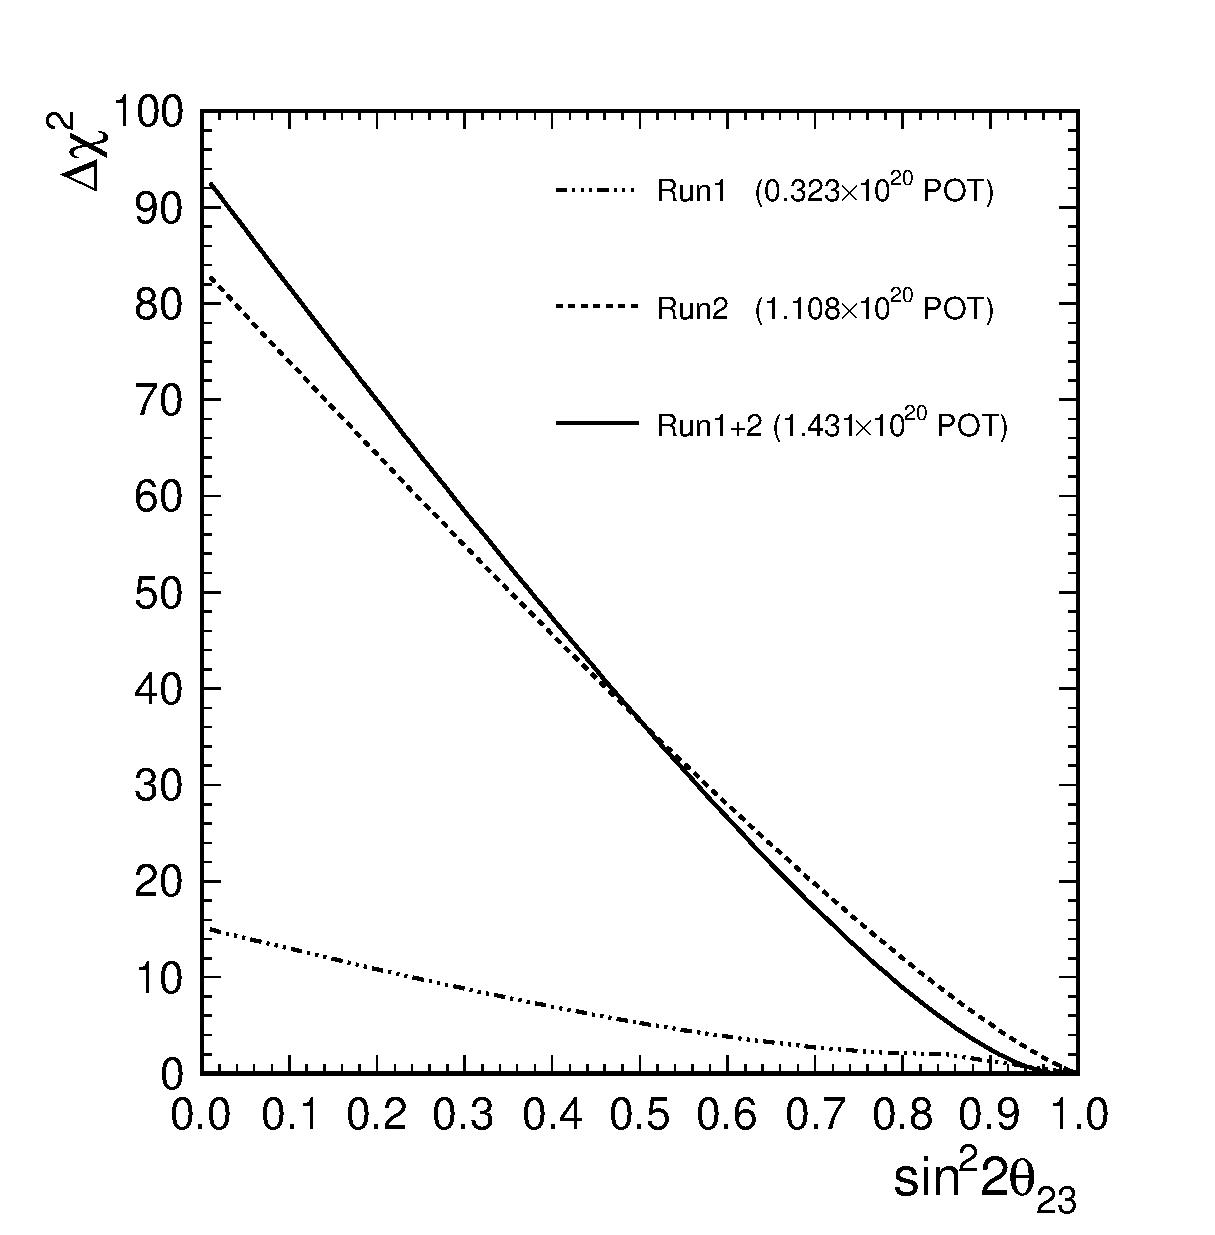
\includegraphics[width=18pc,height=19pc]{./images/fits/neut_marginal_deltachisq_sinsq2theta_3datasets.eps}
\caption{
  The marginalised $\Delta\chi^{2}$ distributions as a function of $sin^{2}2\theta_{23}$ from the 2-flavour
  $\nu_{\mu}$-disappearance fits to the Run1, Run2 and Run1+2 datasets (NEUT).
  All fits were performed in the restricted $|\Delta m^{2}_{23}|$ range from 
  1$\times$10$^{-3}$ $eV^{2}/c^{4}$ to 6$\times$10$^{-3}$ $eV^{2}/c^{4}$.
}
\label{fig:neut_deltachisq_sinsq2theta_3datasets}
\end{minipage}
\end{figure}




\begin{figure*}[htb]
\center
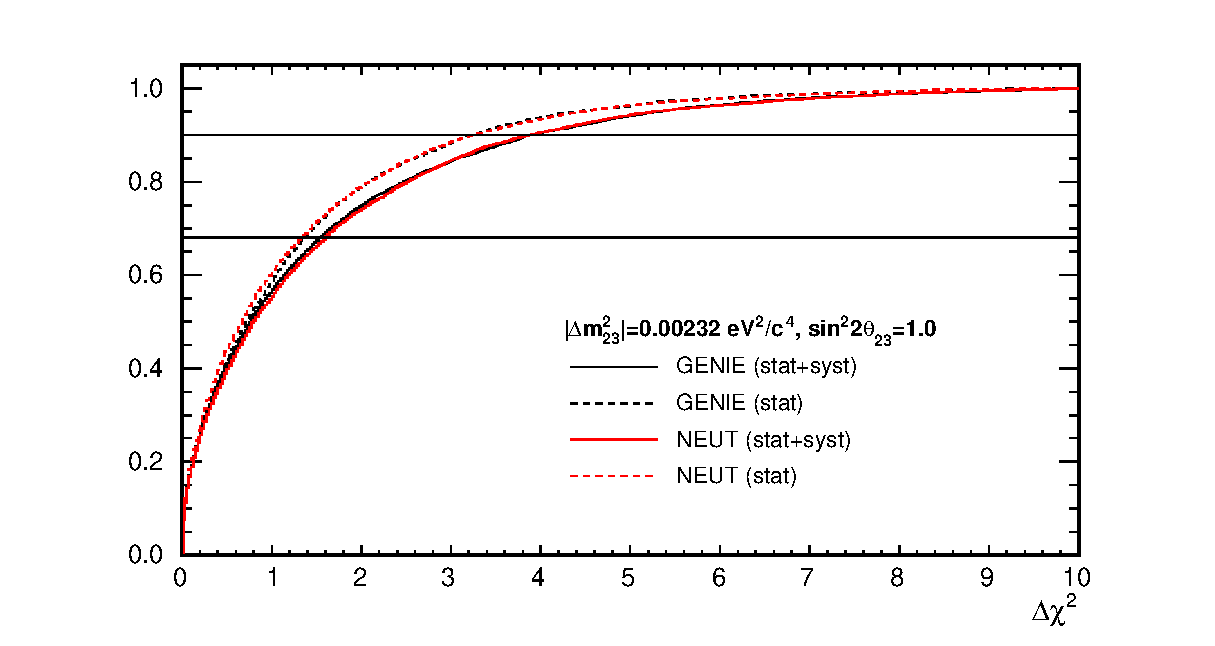
\includegraphics[width=30pc]{./images/feldman_cousins/minos2011_dchisq_cummulative.eps}
\caption{
  Cumulative $\Delta\chi^{2}_{MC}$ distributions (for both NEUT and GENIE) for oscillated toy MC experiments generated
  with $sin^{2}2\theta_{23}$ = 1.0 and $|\Delta m^{2}_{23}|$ = 2.32$\times10^{-3}$ $eV^{2}/c^{4}$.
  The horizontal lines show the 68\% and 90\% levels
  (values of $\Delta\chi^{2}_{critical}$ are the values of $\Delta\chi^{2}_{MC}$ where these horizontal lines
  intersect with the cumulative distributions).
}
\label{fig:minos2011_dchisq_cumulative}
\end{figure*}

